\documentclass[3p, sort&compress]{elsarticle}
\usepackage{titlesec}
\usepackage{typed-checklist}
\titleformat{\paragraph}[runin]{%
    \normalsize\itshape\bfseries}{\theparagraph}{1em}{}
\titlespacing*{\paragraph}{0pt}{%
    3.25ex plus 1ex minus .2ex}{\the\fontdimen2\font}
\usepackage[utf8]{inputenc}
\usepackage{amsmath}
\usepackage{amssymb}{}
\usepackage{amsthm}
\usepackage{enumitem}
\usepackage{lineno, hyperref}
\usepackage{listings}
\usepackage{booktabs}
\usepackage{siunitx}
\usepackage{graphicx}
\usepackage[nameinlink,noabbrev]{cleveref}
\usepackage[draft]{changes}
\usepackage[section]{placeins}
\usepackage[]{algorithm,algcompatible,lipsum}
\usepackage[]{algpseudocode}
\usepackage{scrextend}
\usepackage{changes}

\usepackage{tikz}

%
\modulolinenumbers[1]
\definechangesauthor[color=orange]{SDIV}
\linenumbers
\newdefinition{hypotheses}{Hypothesis}
\newdefinition{assumptions}{Assumptions}
\newdefinition{rmk}{Remark}
\graphicspath{{./Figures/}{./figs/}}
\begin{document}
    %!TEX root = main.tex

% Title footnote mark
% eg: \tnotemark[1]
\tnotemark[1] 

% Title footnote 1.
% eg: \tnotetext[1]{Title footnote text}
\tnotetext[1]{Here the note} 

% First author
%
% Options: Use if required
% eg: \author[1,3]{Author Name}[type=editor,
%       style=chinese,
%       auid=000,
%       bioid=1,
%       prefix=Sir,
%       orcid=0000-0000-0000-0000,
%       facebook=<facebook id>,
%       twitter=<twitter id>,
%       linkedin=<linkedin id>,
%       gplus=<gplus id>]

\author[1,3]{Saul Diaz-Infante}[%
  auid=000,
  bioid=1,
  %prefix=Prof.,
  role=Researcher,
  orcid=0000-0001-9559-1293
]

% Corresponding author indication
\cormark[1]

% Footnote of the first author
\fnmark[1]

% Email id of the first author
\ead{saul.diazinfante@unison/mx}

% URL of the first author
\ead[url]{sauldiazinfantevelasco@wordpress}

% Credit authorship
% eg: \credit{Conceptualization of this study, Methodology, Software}
\credit{Data curation, Writing-Original draft presentation,
  Conceptualization of this study, Methodology, Software, 
  Parameter callibration}

% Address/affiliation
\affiliation[1]{
  organization = {CONACYT-Universida de Sonora},
  addressline = {
    Departamento de Matem\'aticas,
    Universidad de Sonora, Blvd.
    Luis Encinas y Rosales S/N}, 
    city={Hermosillo
  },
%         citysep={}, % Uncomment if no comma needed between city and postcode
  postcode = {83000}, 
  state = {Sonora},
  country = {Mexico}
}

% \author[2]{David Gonzalez-Sanchez}[<options>]

% % Footnote of the second author
% \fnmark[2]

% % Email id of the second author
% \ead{}

% % URL of the second author
% \ead[url]{}

% % Credit authorship
% \credit{}

% % Address/affiliation
% \affiliation[<aff no>]{organization={},
%             addressline={}, 
%             city={},
% %          citysep={}, % Uncomment if no comma needed between city and postcode
%             postcode={}, 
%             state={},
%             country={}}

% % Corresponding author text
% \cortext[1]{Corresponding author}

% % Footnote text
% \fntext[1]{}

% For a title note without a number/mark
%\nonumnote{}
\begin{keywords}
  COVID-19 \sep 
  Optimal Control \sep 
  Lockdown \sep 
  vaccine \sep
  Vaccination \sep
  WHO-SAGE \sep 
  DALYs
\end{keywords}
%!TEX root = main.tex
\begin{abstract}
    We formulate a controlled system of ordinary differential equations, with 
vaccination and lockdown interventions as controls, to simulate the mitigation 
of COVID-19. The performance of the controls is measured through a cost 
functional involving vaccination and lockdown costs as well as the burden of 
COVID19 quantified in DALYs. We calibrate parameters with data from Mexico City 
and Valle de Mexico.  By using differential evolution, we minimize the cost 
functional subject to the controlled system and find optimal policies that are 
constant in time intervals of a given size. The main advantage of these 
policies relies on its practical implementation since the health authority has 
to make only a finite number of different decisions. Our methodology to find 
optimal policies is relatively general, allowing changes in the dynamics, the 
cost functional, or the frequency the policymaker changes actions.
\end{abstract}

\begin{highlights}
	\item 
		Modeling vaccination and lockdown in COVID-19 as an optimal 
		control problem
	\item
		Quantifying desease damages by means of DALYs 
	\item
		Optimal policies in COVID-19 pandemic considering lockdown 
		costs 
	\item
		Solving optimal applied control problems by using Differential Evolution
	\item
		Piecewise optimal policies in optimal control problems
\end{highlights}

    \section{Introduction}
        %!TEX root = main.tex
% 1 definition of the topic plus
%background

    After more than 600 days, we face the devastating consequences of the still
ongoing COVID-19 pandemic. SARS-CoV-2 variants arise, but strict lockdown
is economical-infeasible---particularly in low-income countries like  Mexico.
Despite, the world have now several vaccine developments to fight against this
illness, the uncertainty towards a state similar to our previous normality is
the only matter of fact. In Mexico, healthcare infrastructures are poor, the
national vaccines' rollout still is under progress and limited by the
continuous adjustments required for its administration. Further, despite more
virulent and dangerous coronavirus variants arise, restrictive lockdown
is economically infeasible. Meanwhile, kids and students under isolation need
to retake face-to-face activities to overcome the harder consequences.
Because the most effective strategies available to face this pandemic are
lockdown and vaccination, we suppose that synchronizing these strategies would
improve their mitigation response. Here, we aim to unfold this premise by an
optimal control problem.
%
% 2. Accepted state of the art plus
%problem to be resolved

    On July 2020, the Strategic Advisory Group of Experts (SAGE) on
Immunization Working Group on COVID-19 Vaccines from WHO made public a set of
questions to encourage and direct the efforts of modelling groups to address
the design of vaccination policies \cite{sage2020}. Much of the  resent
development of vaccination models for COVID-19 try to  answer that questions.
We see particularly important topics like the epidemiological aspects of
SARS-CoV-2 and COVID-19, the vaccine landscape and supply-uptake scenarios.
The prioritization of scarce supplies and the economic impact of the regarding
vaccination policies. The first advances answer questions like how many
doses to allocate to each different group according to risk and age to minimize
the burden of COVID-19 or when to intensify the administration doses according
to the Outbreak evolution. However, the modeling of combined strategies like
NPIs and vaccination are under development.

    Our research in this manuscript explores the effect of synchronized Lockdown
and Vaccination interventions, to mitigate the  propagation of COVID-19.
We claim that this combined strategy would improve the mitigation of the
current pandemic and also would protect the economic harsh that implies the
implementation of Lockdowns.

%3 Authors' objectives
    Since health services' response will be limited by the vaccine stock and
logistics costs, implementing in parallel NPIs is imminent. We focus on
formulating and studying via simulation a lockdown-vaccination system by
considering the already announced back to school and vaccines recently approved
by Mexico Health Council. We aim to design a dose administration
schedule subject to a given vaccine stock, that has to be administrated in a
given period, but synchronizing with the release of the isolated
individuals\textemdash as the student population. For this purpose, we
formulate an optimal control problem that minimizes the burden of COVID-19 in
DALYs \cite{WhoDALY}, the cost generated by running the vaccination campaign,
and economic damages due to lockdown.


%4 INTRODUCTION TO LITERATURE
%
    Among the related literature about the mentioned interventions, we see
relevant the following advances. The problem of whom to vaccinate first, when
the number of available shots is limited, has been transformed into an optimal
allocation problem of vaccine doses in \cite{Bubar2020,Matrajt2020,Buckner2020}.
Other papers modeling NPIs as \cite{Naraigh2020,Ullah2020} consider diminishing
of contact rates by reducing mobility or modulating parameters regarding the
generation of new infections by linear controls. Mandal et al. models the
lockdown-quarantine in \cite{Mandal2020} as a control signal, and the authors
of \cite{Weitz2020} propose a shield immunity. Libotte et al. also report in
\cite{Libotte2020} optimal vaccination strategies for COVID-19. Our study takes
the allocation for granted and modulates vaccination and lockdown-release rates
as a combined strategy. Much of recent research in COVID-19 vaccination
consider separately vaccination or lockdown policies, but not synchronized or
balanced with economical implications.

% 6. AUTHORS's CONTRIBUTION
    To the best of our knowledge, this manuscript reports the first piecewise
optimal control model which combine and synchronize lockdown and vaccination
strategies. One of the main features of our model is that we consider piecewise
constant control policies instead of general measurable control policies---also
called permanent controls. Generally,  the control policies in continuous time
are impractical after a sufficiently large time. Since the authorities have to
make different choices permanently, but over discrete periods of time, we
perceive it more natural to deploy piecewise policies. The optimal policies we
find are constant in each interval of time, and hence results more practical and
consistent with reality.

%7. AIM OF THE PRESENTED WORK
    The aim of this contribution is to model and explore scenarios when an
isolated population retake activities face-to-face and then becomes susceptible
to acquire SARS-CoV-2, and at the same time, the rollout of a given vaccine is
under progress. Thus, a decision maker has to balance the release of Lockdown
and the number of vaccines to maximize the mitigation of symptomatic cases and
Deaths related with COVID-19.

% 8 MAIN RESULTS / CONCLUSIONS
    Our simulations suggest that combined and well-synchronized policies of
lockdown-release and vaccination would lead to a better response in the
mitigation of prevalence and deaths due to COVID-19.

% OUTLINE
    After this brief introduction, in \Cref{sec:Covid19_spread}, we formulate
the basic spread model for COVID-19 and calibrate its parameters. Then,
\Cref{sec:vaccination_model} establishes the lockdown-vaccination model and
discusses the regarding reproductive number in \Cref{sec:reproductive_number}.
We describe in \Cref{sec:optimal_controlled} our optimal control problem.
The optimal policies we find, by solving numerically the optimal control
problem, are presented in \Cref{sec:numerical_experiments}.
We conclude with some final comments in \Cref{sec:discussion}.

    \section{Covid-19 spread dynamics}
        \label{sec:Covid19_spread}
        %!TEX root = main.tex
    We split a given population of size $N$ in the basic SEIR
structure with segregated classes according to the manifestation
of symptoms. Let $L, S, E, I_S, I_A, H, R, D$ respectively denote the
class of individuals according to their current state, namely
%
\begin{description}[%
    labelwidth=\widthof{\textbf{Infected-Asymptomatic $(I_A)$}},
    leftmargin=\widthof{\textbf{Infected-Asymptomatic $(I_A)$}},
    align=right%
]
    \item[Lockdown $(L)$:]
        All individuals that have low or null mobility and remain under
        isolation. Thus individuals in this class reduce their contagion 
        probability.
    \item[Susceptible $(S)$:]
        Individuals under risk.
    \item[Exposed $(E)$:]
        Population fraction that hosts SARS-CoV-2 but cannot infect.
    \item[Infected-Symptomatic $(I_S)$:]
        Population infected fraction with symptoms and reported as confirmed
        cases.
    \item[Infected-Asymptomatic $(I_A)$:]
        Infected individuals with transitory or null symptoms and unreported.
    \item[Hospitalized $(H)$:]
        Infected population that requires hospitalization or intensive care.
    \item[Recover or removed $(R)$:]
        Population that recovers from infection and develops partial immunity.
    \item[Death $(D)$:]
        Population fraction that died due to COVID-19.
\end{description}
%
To fit data of cumulative reported symptomatic cases, we
postulate the counter state $Y_{I_S}$ and make the following assumptions.
%
%
\begin{assumptions}
    According to above compartment description, we made the following
    hypotheses.
    \begin{enumerate}[label={(A-\arabic*)}]
        \item
            We suppose that at least \SI{30}{\percent} of the population is
            locked down and a fraction of this class eventually moves
            to the susceptible compartment at rate $\delta_L$.
        \item
            Force infection is defined as the probability of acquiring COVID-19
            given the contact with a symptomatic or asymptomatic individual.
            Thus we normalize with respect to alive population population
            $
                N^{\star}
            $.
        \item
            Susceptible individuals become
            exposed\textemdash but not infectious\textemdash
            % exposed individuals
            %host the virus but can not transmit it.
            when they are in contact with asymptomatic or symptomatic
            individuals. Thus $\beta_S$ and $\beta_A$ denote the
            probabilities of being infectious given the contact with a 
            symptomatic orasymptomatic infectious individuals, respectively.
        \item
            After a period of latency  $1/\kappa = \SI{5.1}{days}$, an
            exposed individual becomes infected. Being $p$ the probability of
            developing symptoms and $(1-p)$ the probability of becoming infectious
            but asymptomatic. Thus $p\kappa E$ denotes the
            exposed individuals that become infectious and develop symptoms.
        \item
            Asymptomatic individuals do not die or stay in the hospital.
        \item
            A fraction $\mu_{H}$ of symptomatic individuals
            dies due to COVID-19 without hospitalization.
        %\item
    \end{enumerate}
\end{assumptions}

\begin{figure*}[tbh]
    \centering
      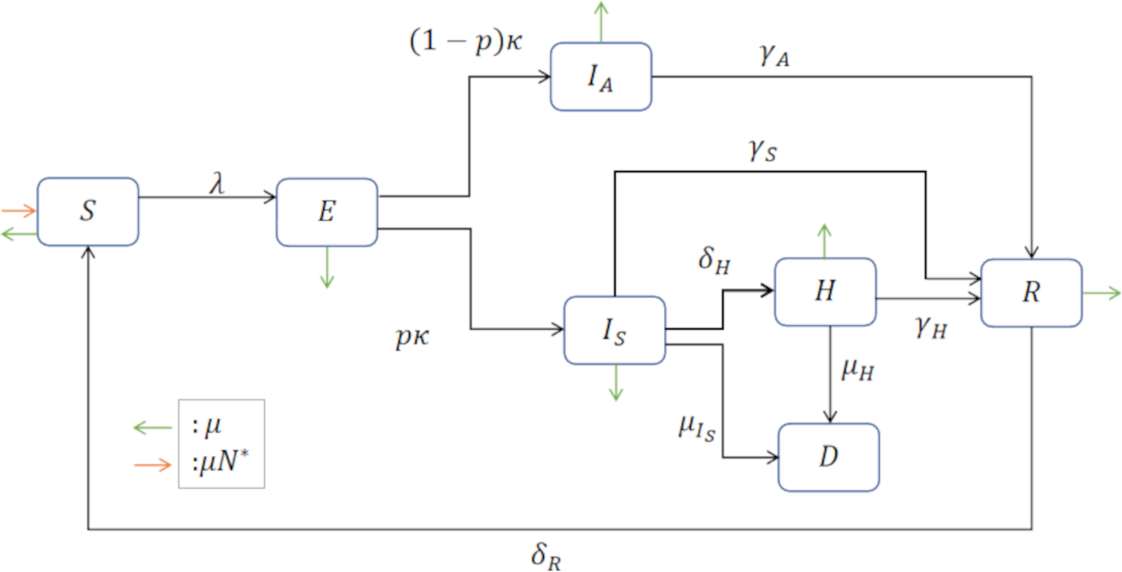
\includegraphics[scale=0.7, keepaspectratio]{Diagram_no_Vaccination.pdf}
        \caption{
            Compartmental diagram of COVID-19 transmission dynamics. 
            Consider the class: Susceptible $(S)$, exposed $(E)$, symptomatic 
            infected $(I_S)$, asymptomatic infected $(I_A)$, recovered $(R)$, 
            death $(D)$ and vaccinated $(V)$ individuals. It is important to 
            mention that $I_{S}$ represents the proportion of symptomatic 
            individuals who will later report to some health medical center.
        }
    \label{fig:diagramnolockdownandVacc}
\end{figure*}

Thus we formulate the following Ordinary Differential Equation (ODE), see
\Cref{fig:diagramnolockdownandVacc}, to complete the underlying description.
\begin{equation}
	\label{eqn:base_dynamics}
    \begin{aligned}
        S' & =
            \mu N^\star + \delta_R R - (\lambda + \mu)
            S,
        \\
        E' & =
            \lambda (\epsilon L + S) - (\kappa + \mu) E,
        \\
        I_S' & =
            p \kappa E -
            (\gamma_S +
                \delta_H +
                \mu_{I_S} +
                \mu) I_S,
        \\
        I_A' &=
            (1 - p) \kappa E - (\gamma_A + \mu) I_A,
        \\
        H' &=
            \delta_H I_S - (\gamma_H + \mu_H + \mu) H,
        \\
        R' & =
            \gamma_S I_S + \gamma_A I_A + \gamma_H H - (\delta_R + \mu) R,
        \\
        D' &=
            \mu_{I_S} I_S + \mu_H H,
        \\
        \frac{dY_{I_S}}{dt} &  = p \kappa E,
        \\
        \lambda &:=
            \frac{\beta_A I_A + \beta_S I_S}{N^{\star}},
        \\
        N^{\star}(t) &=
            L + S + E +
            I_S + I_A +
            H + R .
    \end{aligned}
\end{equation}
%
\begin{figure}
    \begin{center}
        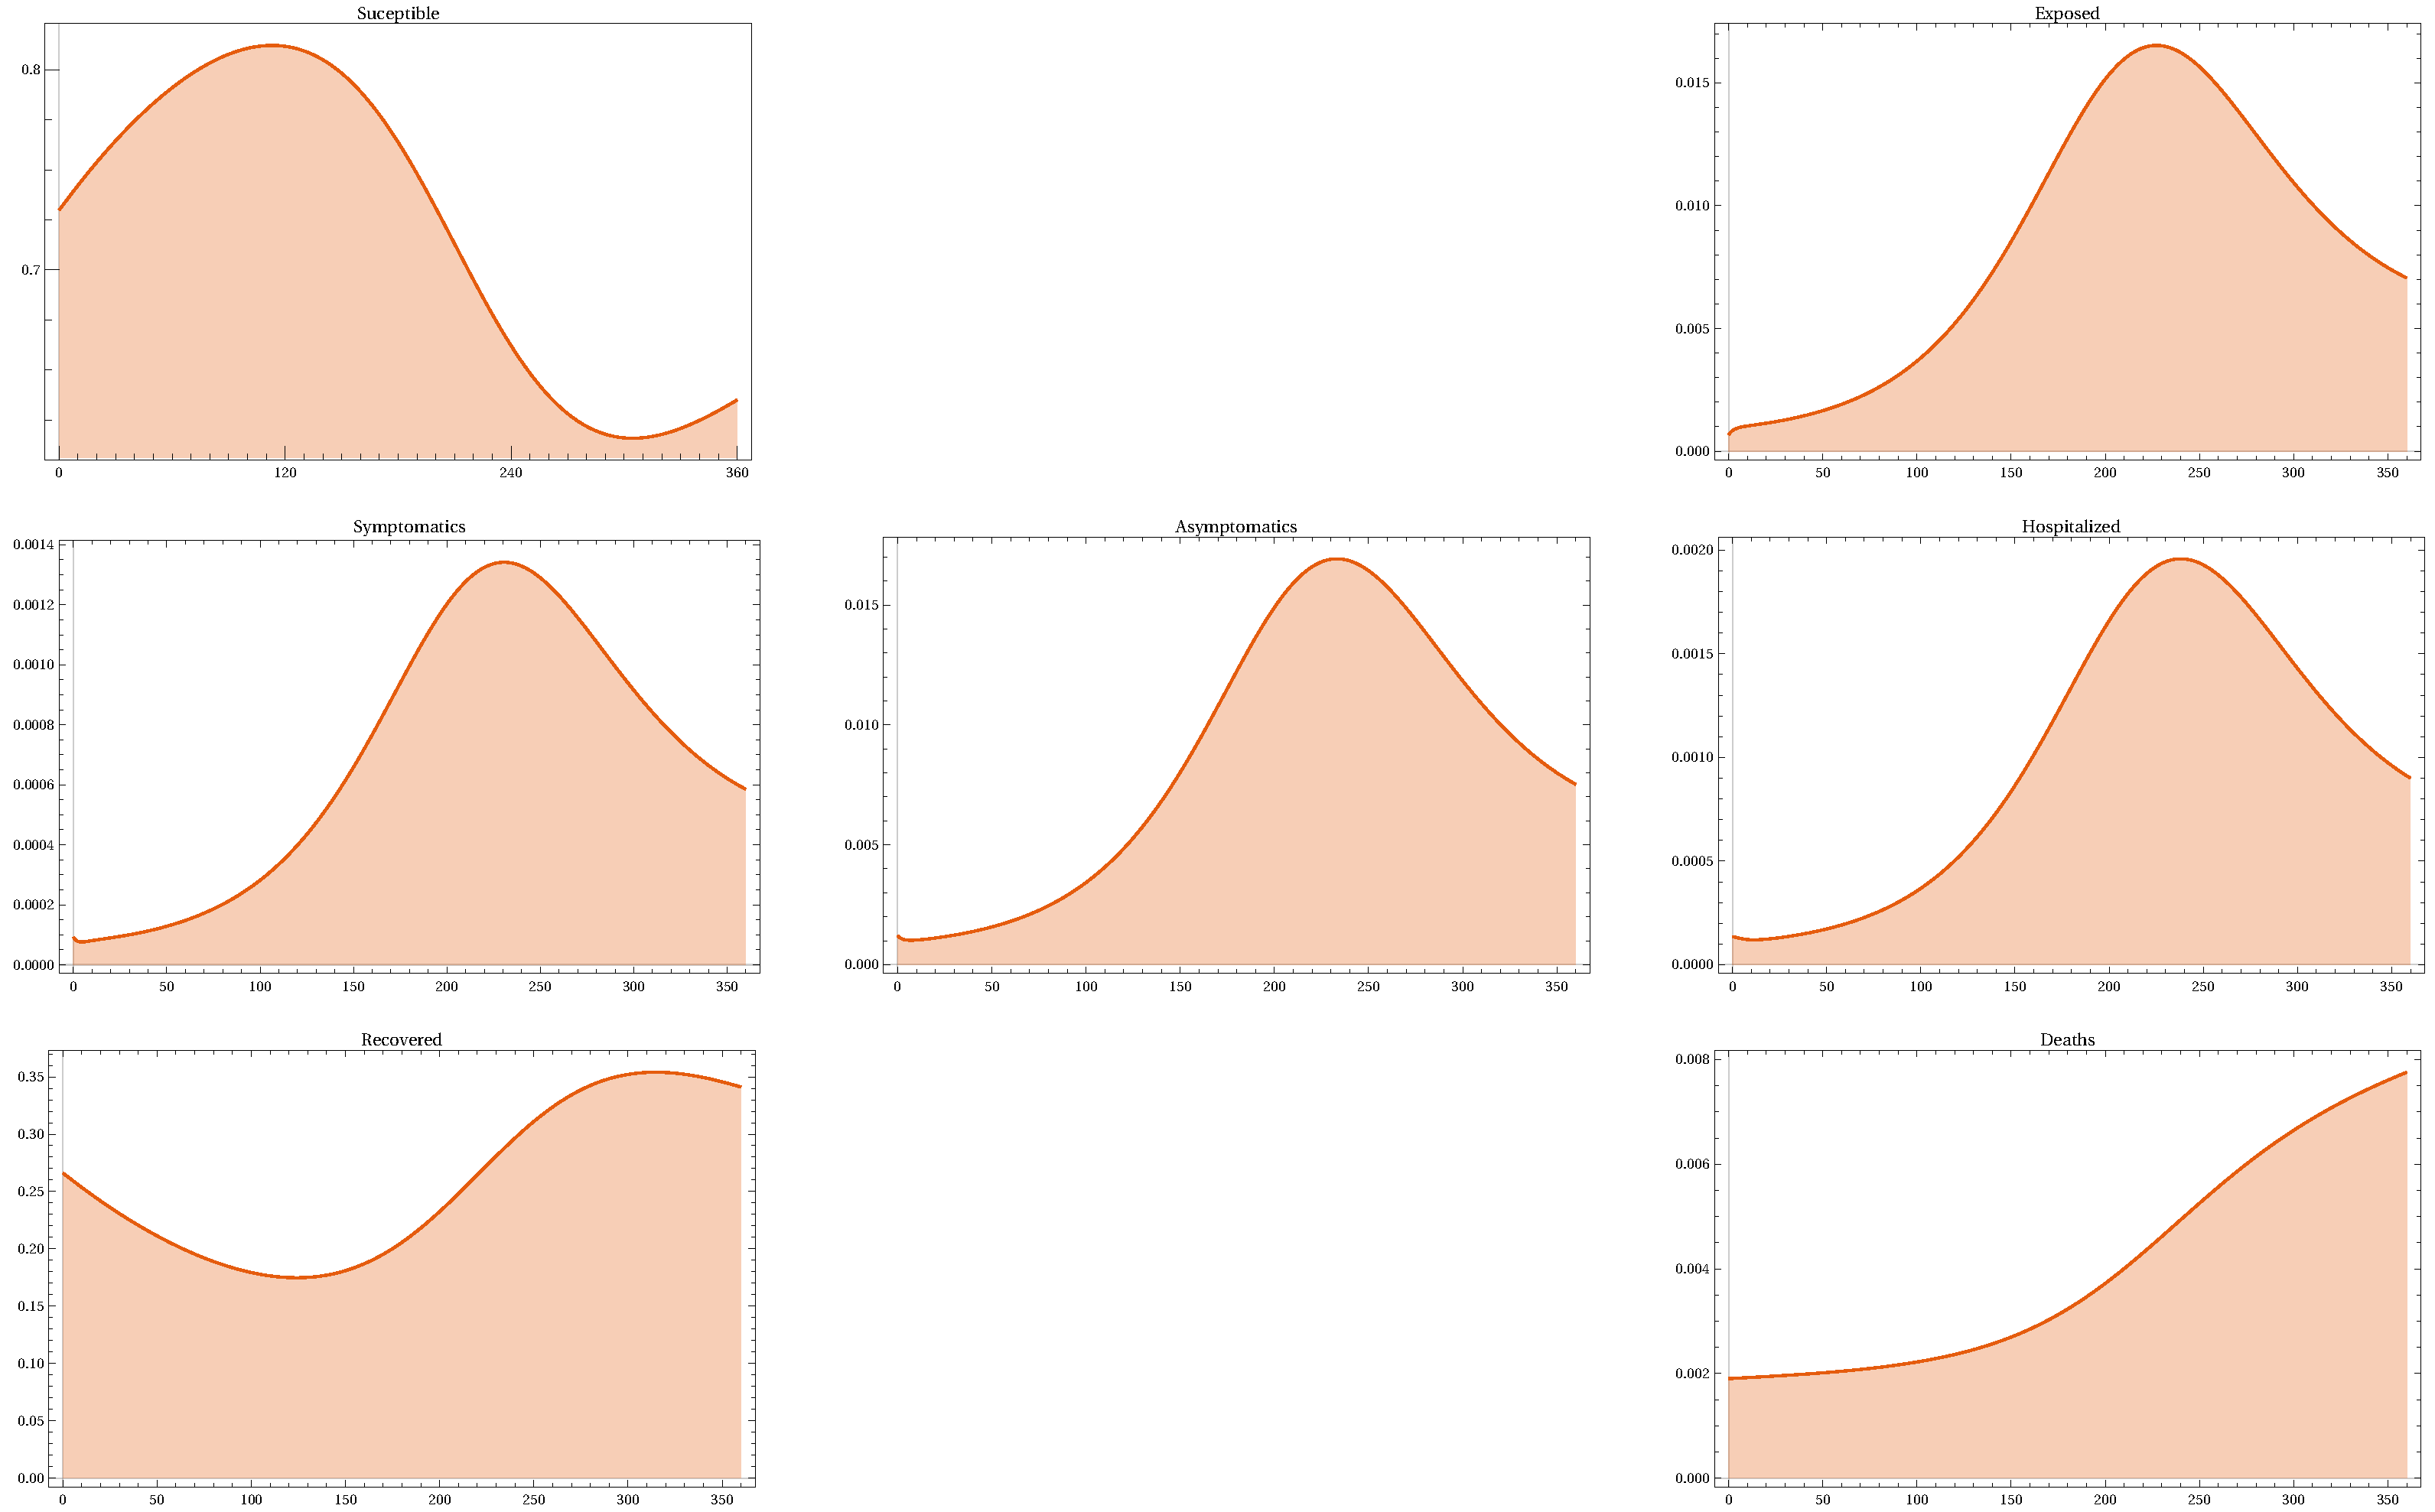
\includegraphics[scale=0.25,
        keepaspectratio]{no_contraled_dynamics}
    \end{center}
    \caption{
        Spreed dynamics of COVID-19 according to model in
        \Cref{eqn:base_dynamics}.
    }
    \label{fig:base_dynamics}
\end{figure}

    We display in \Cref{fig:base_dynamics} a typical evolution of this COVID-19 spreed dynamics.
\Cref{tbl:dynamics_base_parameters} encloses notation and reference values.
%
\begin{table*}[h!]
	\centering
	\begin{tabular}{>{\centering}%
        p{0.2\textwidth}%
        p{0.4\textwidth}
    }
    \toprule
		\textbf{Parameter} & \textbf{Description}
  	\\
  	\midrule
		$\mu$ &
			Death rate
		\\
        $\beta_S$ &
        	Infection rate between susceptible and symptomatic infected
		\\
        $\beta_A$ &
        	Infection rate between susceptible and asymptomatic infected
		\\
        $\lambda_V$ &
        	Vaccination rate
		\\
        $\delta_{V}^{-1}$ &
        Vaccine-induced immunity
		\\
        $\varepsilon$ &
        	Vaccine efficacy
		\\
        $\kappa^{-1}$ &
        	Average incubation time
        \\
		$p$ &
			New asymptomatic generation proportion
		\\
	    $\theta$ &
        	Proportion of suceptible individuals under lockdown
        \\
        $\gamma_{S}^{-1}$ &
        	Average time of symptomatic recovery
        \\
		$\gamma_{A}^{-1}$ &
			Recovery average time of asymptomatic individuals
		\\
		$\gamma_{H}^{-1}$ &
			Recovery average time by hospitalization
		\\
        $\delta_{R}^{-1}$ &
        	Natural immunity
  		\\
  		$\delta_{H}$ &
        	Infected symptomatic hospitalization rate
  		\\
  	\bottomrule
	\end{tabular}
		\caption{
			Parameters definition of model in
			\Cref{eqn:base_dynamics}.}
    \label{tbl:dynamics_base_parameters}
\end{table*}
%
\begin{figure*}[htb]
    \centering
    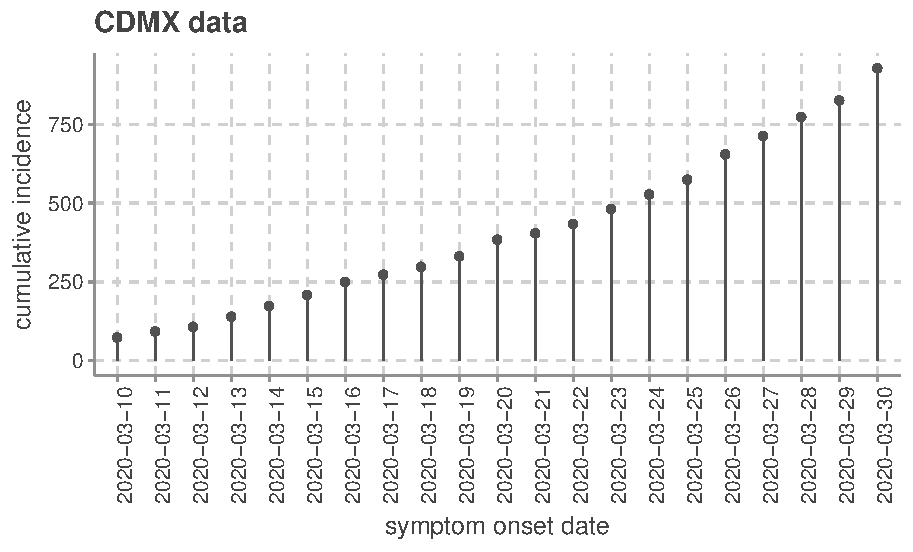
\includegraphics[scale=0.8, keepaspectratio]{Figures/cdmx_input_data}
    \caption{%
        Cumulative new symptomatic and confirmed COVID19 reported cases from
        Ciudad de Mexico and Valle de Mexico
        \cite{cdmxDATA} between March, 10, to March 30 of
        2020.
        \href{https://plotly.com/~AdrianSalcedo/48/}{%
		https://plotly.com/~AdrianSalcedo/48/}
	}
    \label{fig:data_CDMX}
\end{figure*}
%

        \subsection{Parameter calibration}
            %!TEX root = main.tex
\begin{figure*}[htb]
    \centering
    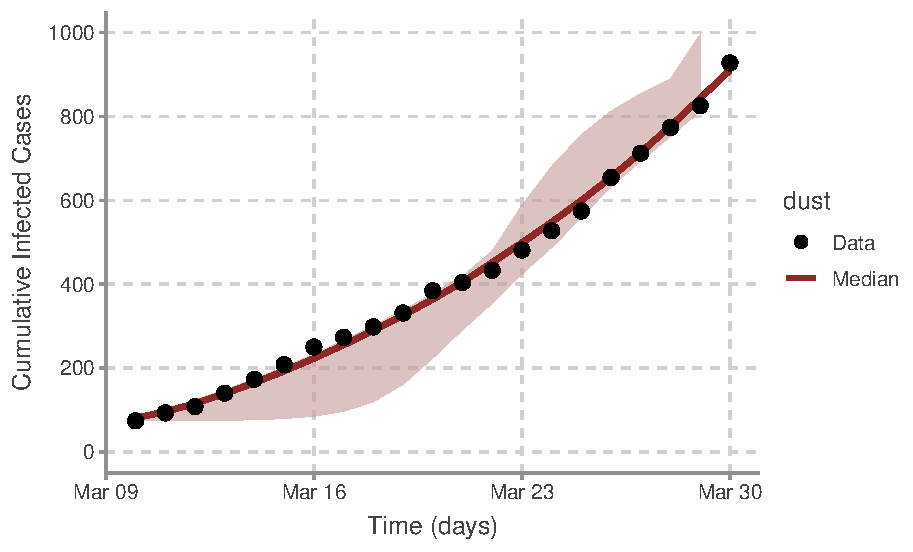
\includegraphics[scale=0.7, keepaspectratio]{./cdmx_CIs_data_begining_fit}
    \caption{%
        Fit of daily new cases of Mexico city
        during exponential growth.
    }
    \label{fig:data_CDMX_fitting}
\end{figure*}
%
%\paragraph{Bayesian estimation}
We calibrate parameters of our base dynamics
\eqref{eqn:base_dynamics} via Multi Chain Monte Carlo (MCMC).
To this end, we assume that the cumulative
incidence of new infected symptomatic cases $Y_{I_S}$
follows a Poisson distribution with mean 
$$
    \lambda_t = 
        \int_{0} ^ t
        p \kappa E.
$$ 
%

    Following ideas from \cite{Acuna2020} we postulate priors for 
$p$ and $\kappa$ and count the cumulative reported-confirmed cases in 
the CDMX-Valle de Mexico database \cite{cdmxDATA}. We fix a time window
to enclose the growth face of the firs wave.
\begin{equation}
    \label{eqn:boservation_model}
    \begin{aligned}
        Y_t & \sim \text{Poisson}(\lambda_t),
        \\
        \lambda_t
        &=
        \int_{0}^t p \kappa E ,
        \\
        & p \sim \text{Uniform} (0.3, 0.8),
        \\
        & \kappa \sim \text{Gamma}(10, 50).
    \end{aligned}
\end{equation}
%
Using Van den Driessche's \cite{Van2002} definition of reproductive number
we obtain
\begin{equation*}
    \label{eqn:reproductive_number}
    \begin{aligned}
        R_0 :=
        &
        \frac{\kappa}{(\kappa + \mu)(\delta_L + \mu)}
        \left(
            \mu R_1 + \delta_L
        \right)
        \left[
            \frac{p\beta_S}{R_2}
            +\frac{(1 - p) \beta_A}{\gamma_A+\mu}
        \right],
    \\
    \text{where} &
    \\
        R_1 &= 1 - \theta(1 - \epsilon),
    \\
        R_2 &= \mu + \delta_H + \gamma_S + \mu_{I_{S}}.
    \end{aligned}
\end{equation*}

\Cref{fig:data_CDMX} displays data of cumulative confirmed cases
of COVID-19 in Mexico city, and \Cref{fig:data_CDMX_fitting} displays 
the fitted curve
of our model in \Cref{eqn:base_dynamics,eqn:boservation_model}.
\Cref{tbl:parameters_values} encloses estimated parameters to this
setting.

  \begin{table*}
    \centering
    \begin{tabular}{@{}llr@{}}
    \toprule
        Parameter
        &   \centering{Median}
        &   Reference
        \\
        \midrule
          $q_r$, $\epsilon$
            &
              \num{.4}\textsuperscript{$\mathsection$}, 
              \num{.3}\textsuperscript{$\mathsection$}, 
              \num{.1}\textsuperscript{$\mathsection$}
            &
              
        \\
            $\beta_S$
            & $q_r \times \num{8.690483e-01}$\textsuperscript{$\mathsection$}
            & 
        \\
            $\beta_A$
            & $q_r \times \num{7.738431e-01}$\textsuperscript{$\mathsection$}
            & 

        \\
            $\kappa$
            & \num{0.19607843}\textsuperscript{$\dagger$}
            & 
        \\
            $p$
            & \num{0.1213}\textsuperscript{$\dagger$}
            & 
        \\
          $\theta$
          & \num{0.2},
          & this study
        \\
          $\delta_L$
          & \num{0.04}
          & postulated
        \\
            $\delta_H$
            &\num{0.2}\textsuperscript{$\dagger$}
            & 
        \\
          $\delta_V$
          &\num{ 0.0027397260273972603}
          & Assumed ($\delta_V ^{-1} = \SI{2}{years}$)
        \\
        &&

        \\
          $\delta_R$
          & \num{0.00555556}
          & Assumed($\delta_R^{-1} \approx \SI{180}{days}$)
        \\
            $\mu$
            & \num{ 3.913894e-05}\textsuperscript{$\dagger$}
            & 
        \\
            $\mu_{I_S}$
            & \num{0.0004}\textsuperscript{$\dagger$}
            & 
        \\
            $\mu_{H}$
            & \num{0.01632}
            & \cite{Zhao2020}
        \\
            $\gamma_S$
            & \num{0.09250694}\textsuperscript{$\dagger$}
            & 
        \\
             $\gamma_A$
             & \num{0.16750419}\textsuperscript{$\dagger$}
             &
        \\
           $\gamma_H$
            & \num{5.079869e-01}\textsuperscript{$\dagger$}
            &
        \\
          $\lambda_V$
          &  \num{0.00061135}
          & Assumed
        \\
          $\varepsilon$
          & \num{0.7}, \num{0.9}, \num{0.95}
          & \cite{cnn_health_2020, reuters2020,cnn_health_2020b}
        \\
        \midrule
            $N$
             & \num{26446435}
             & \cite{conavi2020}
        \\
            $L_0$
            & \num{0.26626009702112796}\textsuperscript{$\ddagger$}
            & 
        \\
            $S_0$
             & \num{0.463606046009872}\textsuperscript{$\ddagger$}
             &
        \\
            $E_0$
             & \num{0.00067033}\textsuperscript{$\ddagger$}
             &
        \\
            $I_{S_0}$
            & \num{9.283e-05}\textsuperscript{$\ddagger$}
            &
        \\
            $I_{A_0}$
            & \num{0.00120986}\textsuperscript{$\ddagger$}
            &
        \\
            $H_0$
            & \num{1.34157969e-04}\textsuperscript{$\ddagger$}
            &
        \\
            $R_0$
            & \num{2.66125939e-01}\textsuperscript{$\ddagger$}
            &
        \\
            $D_0$
            & \num{0.00190074}\textsuperscript{$\ddagger$}
            &
        \\
            $X_{vac}^0$
            & 0.0\textsuperscript{$\mathsection$}
            &
        \\
            $V_0$
            & 0.0\textsuperscript{$\mathsection$}
            &
        \\
            $Y_{I_S} ^ 0$ &
            \num{0.12258164}\textsuperscript{$\ddagger$}
            &
        \\
        \\
            $B$
        &
            \num{0.0003592166581242425}
        &
            $
                \displaystyle
                \SI{9500}{beds} / {N}
            $
        \\
          $a_{I_S}$
            & \num{0.0020127755438256486}\textsuperscript{$\star$}
            &
        \\
          $a_{H}$
            & \num{0.001411888738103725}\textsuperscript{$\star$},
            &
        \\
            $a_D$
            & \num{7.25}\textsuperscript{$\star$}
            &
        \\
        \bottomrule
    \end{tabular}
    \caption{
        Model parameters. (\textsuperscript{$\dagger$}) Values based 
        mainly in \cite{Zhao2020, Ferguson2020}. 
        (\textsuperscript{$\ddagger$}) Estimated.
        (\textsuperscript{$\mathsection$}) 
        This study. (\textsuperscript{$\star$})
        From \cite{Jo2020}.
    } \label{tbl:parameters_values}
\end{table*}
    \section{Imperfect-preventive COVID-19 vaccination}
        \label{sec:vaccination_model}
        %!TEX root = main.tex
%
\begin{assumptions}
     According to COVID-19 dynamics \Cref{eqn:base_dynamics}, we
     made the following modeling hypotheses about the regarding vaccine.
     \begin{enumerate}[label={\textbf{(VH-\arabic*)}}]
        \item
            Vaccine is preventive and only reduce susceptibility.
            
        \item
            The vaccination camping omits testing to detect seroprevalence.
            Thus Exposed, Infected Asymptomatic and Recovered Asymptomatic
            individuals are undetected but would obtain a vaccine dose
            \textemdash which in this model represents a waste of resources
        \item
            Individuals under lockdown are also vaccinated
        \item
            The vaccine is leaky and with efficacy $\epsilon \in[0.7, .975]$
        \item   
            Vaccine induced immunity last \SI{2}{years}
        \item   
            Natural immunity last a period of \SI{180}{days} 
     \end{enumerate}
\end{assumptions}
\begin{figure*}[tbh]
    \centering
      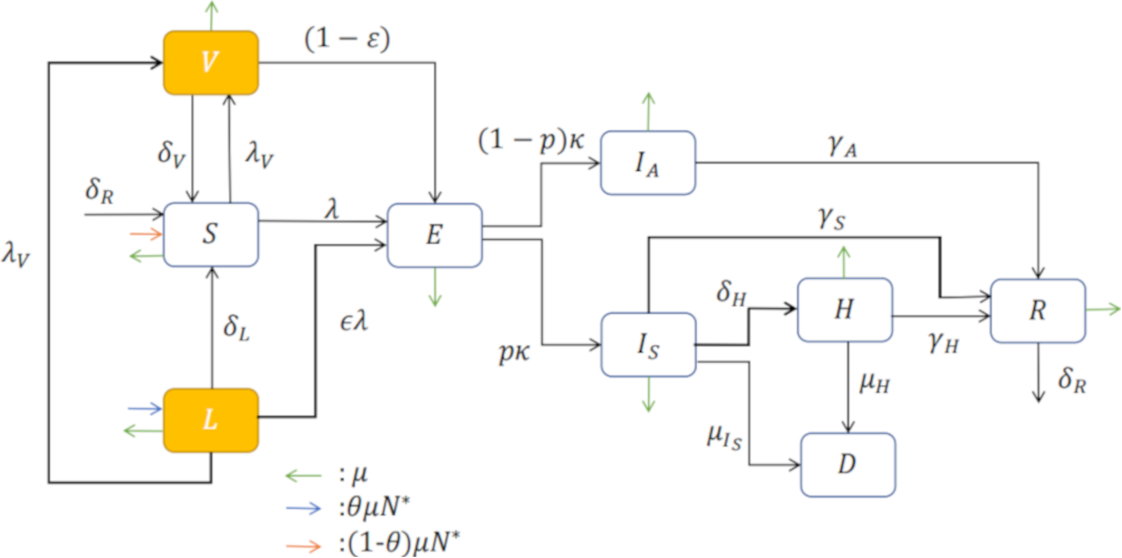
\includegraphics[scale=0.7, keepaspectratio]{Diagram_Vaccination.pdf}
    %

\tikzset{every picture/.style={line width=0.75pt}} %set default line width to 0.75pt        

\begin{tikzpicture}[x=0.75pt,y=0.75pt,yscale=-0.8,xscale=0.8]
%uncomment if require: \path (0,391); %set diagram left start at 0, and has height of 391

%Rounded Rect [id:dp9338258576556762] 
\draw   (40,138) .. controls (40,133.58) and (43.58,130) .. (48,130) -- (102,130) .. controls (106.42,130) and (110,133.58) .. (110,138) -- (110,162) .. controls (110,166.42) and (106.42,170) .. (102,170) -- (48,170) .. controls (43.58,170) and (40,166.42) .. (40,162) -- cycle ;
%Rounded Rect [id:dp03550846434827437] 
\draw   (161,138) .. controls (161,133.58) and (164.58,130) .. (169,130) -- (223,130) .. controls (227.42,130) and (231,133.58) .. (231,138) -- (231,162) .. controls (231,166.42) and (227.42,170) .. (223,170) -- (169,170) .. controls (164.58,170) and (161,166.42) .. (161,162) -- cycle ;
%Rounded Rect [id:dp2096597210016533] 
\draw   (299.5,78) .. controls (299.5,73.58) and (303.08,70) .. (307.5,70) -- (361.5,70) .. controls (365.92,70) and (369.5,73.58) .. (369.5,78) -- (369.5,102) .. controls (369.5,106.42) and (365.92,110) .. (361.5,110) -- (307.5,110) .. controls (303.08,110) and (299.5,106.42) .. (299.5,102) -- cycle ;
%Rounded Rect [id:dp4192775592826552] 
\draw   (299.5,197.5) .. controls (299.5,193.08) and (303.08,189.5) .. (307.5,189.5) -- (361.5,189.5) .. controls (365.92,189.5) and (369.5,193.08) .. (369.5,197.5) -- (369.5,221.5) .. controls (369.5,225.92) and (365.92,229.5) .. (361.5,229.5) -- (307.5,229.5) .. controls (303.08,229.5) and (299.5,225.92) .. (299.5,221.5) -- cycle ;
%Rounded Rect [id:dp9412674774350195] 
\draw   (580.5,197.5) .. controls (580.5,193.08) and (584.08,189.5) .. (588.5,189.5) -- (642.5,189.5) .. controls (646.92,189.5) and (650.5,193.08) .. (650.5,197.5) -- (650.5,221.5) .. controls (650.5,225.92) and (646.92,229.5) .. (642.5,229.5) -- (588.5,229.5) .. controls (584.08,229.5) and (580.5,225.92) .. (580.5,221.5) -- cycle ;
%Rounded Rect [id:dp7750331540351684] 
\draw   (439,288.33) .. controls (439,283.92) and (442.58,280.33) .. (447,280.33) -- (501,280.33) .. controls (505.42,280.33) and (509,283.92) .. (509,288.33) -- (509,312.33) .. controls (509,316.75) and (505.42,320.33) .. (501,320.33) -- (447,320.33) .. controls (442.58,320.33) and (439,316.75) .. (439,312.33) -- cycle ;
%Rounded Rect [id:dp22729858034129236] 
\draw   (439,198) .. controls (439,193.58) and (442.58,190) .. (447,190) -- (501,190) .. controls (505.42,190) and (509,193.58) .. (509,198) -- (509,222) .. controls (509,226.42) and (505.42,230) .. (501,230) -- (447,230) .. controls (442.58,230) and (439,226.42) .. (439,222) -- cycle ;
%Straight Lines [id:da8056305543799926] 
\draw    (109.33,150.17) -- (159.33,149.37) ;
\draw [shift={(161.33,149.33)}, rotate = 539.0799999999999] [color={rgb, 255:red, 0; green, 0; blue, 0 }  ][line width=0.75]    (10.93,-3.29) .. controls (6.95,-1.4) and (3.31,-0.3) .. (0,0) .. controls (3.31,0.3) and (6.95,1.4) .. (10.93,3.29)   ;
%Straight Lines [id:da2787683579538649] 
\draw    (230.78,149.33) -- (265.67,149.17) ;
%Straight Lines [id:da21916666537860907] 
\draw    (265.67,89.17) -- (297.67,89.32) ;
\draw [shift={(299.67,89.33)}, rotate = 180.28] [color={rgb, 255:red, 0; green, 0; blue, 0 }  ][line width=0.75]    (10.93,-3.29) .. controls (6.95,-1.4) and (3.31,-0.3) .. (0,0) .. controls (3.31,0.3) and (6.95,1.4) .. (10.93,3.29)   ;
%Straight Lines [id:da8438200798129222] 
\draw    (265.67,88.6) -- (265.67,209.17) ;
%Straight Lines [id:da7337155371803761] 
\draw    (265.67,209.17) -- (297.67,209.32) ;
\draw [shift={(299.67,209.33)}, rotate = 180.28] [color={rgb, 255:red, 0; green, 0; blue, 0 }  ][line width=0.75]    (10.93,-3.29) .. controls (6.95,-1.4) and (3.31,-0.3) .. (0,0) .. controls (3.31,0.3) and (6.95,1.4) .. (10.93,3.29)   ;
%Straight Lines [id:da509274682669141] 
\draw    (369.43,204) -- (424.2,204.39) -- (437.2,204.49) ;
\draw [shift={(439.2,204.5)}, rotate = 180.41] [color={rgb, 255:red, 0; green, 0; blue, 0 }  ][line width=0.75]    (10.93,-3.29) .. controls (6.95,-1.4) and (3.31,-0.3) .. (0,0) .. controls (3.31,0.3) and (6.95,1.4) .. (10.93,3.29)   ;
%Straight Lines [id:da3183759306298827] 
\draw    (405,299.5) -- (437,299.34) ;
\draw [shift={(439,299.33)}, rotate = 539.72] [color={rgb, 255:red, 0; green, 0; blue, 0 }  ][line width=0.75]    (10.93,-3.29) .. controls (6.95,-1.4) and (3.31,-0.3) .. (0,0) .. controls (3.31,0.3) and (6.95,1.4) .. (10.93,3.29)   ;
%Straight Lines [id:da6861028849351065] 
\draw    (370,214) -- (404.8,214.1) ;
%Straight Lines [id:da9190171216881116] 
\draw    (404.8,214.1) -- (405,300) ;
%Straight Lines [id:da03313994658252273] 
\draw    (508.33,219.33) -- (565.2,219.39) -- (578.78,219.34) ;
\draw [shift={(580.78,219.33)}, rotate = 539.78] [color={rgb, 255:red, 0; green, 0; blue, 0 }  ][line width=0.75]    (10.93,-3.29) .. controls (6.95,-1.4) and (3.31,-0.3) .. (0,0) .. controls (3.31,0.3) and (6.95,1.4) .. (10.93,3.29)   ;
%Straight Lines [id:da6934604539767528] 
\draw    (474.33,230) -- (474.76,278.22) ;
\draw [shift={(474.78,280.22)}, rotate = 269.49] [color={rgb, 255:red, 0; green, 0; blue, 0 }  ][line width=0.75]    (10.93,-3.29) .. controls (6.95,-1.4) and (3.31,-0.3) .. (0,0) .. controls (3.31,0.3) and (6.95,1.4) .. (10.93,3.29)   ;
%Straight Lines [id:da6916456040068684] 
\draw    (369,89.17) -- (614.6,90) ;
%Straight Lines [id:da7246498566982733] 
\draw    (614.6,90) -- (615.32,187.17) ;
\draw [shift={(615.33,189.17)}, rotate = 269.58] [color={rgb, 255:red, 0; green, 0; blue, 0 }  ][line width=0.75]    (10.93,-3.29) .. controls (6.95,-1.4) and (3.31,-0.3) .. (0,0) .. controls (3.31,0.3) and (6.95,1.4) .. (10.93,3.29)   ;
%Straight Lines [id:da5396778112959429] 
\draw    (335,139.17) -- (335,189.5) ;
%Straight Lines [id:da7180507787496266] 
\draw    (334.2,138.8) -- (530.8,139.2) ;
%Straight Lines [id:da3365589163505732] 
\draw    (531,199.71) -- (578,200.18) ;
\draw [shift={(580,200.2)}, rotate = 180.57] [color={rgb, 255:red, 0; green, 0; blue, 0 }  ][line width=0.75]    (10.93,-3.29) .. controls (6.95,-1.4) and (3.31,-0.3) .. (0,0) .. controls (3.31,0.3) and (6.95,1.4) .. (10.93,3.29)   ;
%Straight Lines [id:da7818385183529692] 
\draw    (530.8,139.2) -- (531,199.71) ;
%Straight Lines [id:da7484740849372823] 
\draw    (75,338.67) -- (76.19,171.5) ;
\draw [shift={(76.2,169.5)}, rotate = 450.41] [color={rgb, 255:red, 0; green, 0; blue, 0 }  ][line width=0.75]    (10.93,-3.29) .. controls (6.95,-1.4) and (3.31,-0.3) .. (0,0) .. controls (3.31,0.3) and (6.95,1.4) .. (10.93,3.29)   ;
%Straight Lines [id:da29835177923282885] 
\draw    (75,338.67) -- (615.67,340) ;
%Straight Lines [id:da7139155616312535] 
\draw    (615.33,229.67) -- (615.67,340) ;
%Straight Lines [id:da20994732667721105] 
\draw [color={rgb, 255:red, 245; green, 166; blue, 35 }  ,draw opacity=1 ][fill={rgb, 255:red, 65; green, 117; blue, 5 }  ,fill opacity=1 ]   (10.25,139.04) -- (38,139) ;
\draw [shift={(40,139)}, rotate = 539.9200000000001] [color={rgb, 255:red, 245; green, 166; blue, 35 }  ,draw opacity=1 ][line width=0.75]    (10.93,-3.29) .. controls (6.95,-1.4) and (3.31,-0.3) .. (0,0) .. controls (3.31,0.3) and (6.95,1.4) .. (10.93,3.29)   ;
%Straight Lines [id:da9409632697808414] 
\draw [color={rgb, 255:red, 65; green, 117; blue, 5 }  ,draw opacity=1 ]   (39.75,159.29) -- (12.25,159.29) ;
\draw [shift={(10.25,159.29)}, rotate = 360] [color={rgb, 255:red, 65; green, 117; blue, 5 }  ,draw opacity=1 ][line width=0.75]    (10.93,-3.29) .. controls (6.95,-1.4) and (3.31,-0.3) .. (0,0) .. controls (3.31,0.3) and (6.95,1.4) .. (10.93,3.29)   ;
%Straight Lines [id:da671739616587531] 
\draw [color={rgb, 255:red, 65; green, 117; blue, 5 }  ,draw opacity=1 ]   (195,169.79) -- (195.23,197.54) ;
\draw [shift={(195.25,199.54)}, rotate = 269.52] [color={rgb, 255:red, 65; green, 117; blue, 5 }  ,draw opacity=1 ][line width=0.75]    (10.93,-3.29) .. controls (6.95,-1.4) and (3.31,-0.3) .. (0,0) .. controls (3.31,0.3) and (6.95,1.4) .. (10.93,3.29)   ;
%Straight Lines [id:da4612478738976049] 
\draw [color={rgb, 255:red, 65; green, 117; blue, 5 }  ,draw opacity=1 ]   (335.25,229.79) -- (335.48,257.54) ;
\draw [shift={(335.5,259.54)}, rotate = 269.52] [color={rgb, 255:red, 65; green, 117; blue, 5 }  ,draw opacity=1 ][line width=0.75]    (10.93,-3.29) .. controls (6.95,-1.4) and (3.31,-0.3) .. (0,0) .. controls (3.31,0.3) and (6.95,1.4) .. (10.93,3.29)   ;
%Straight Lines [id:da6463966696699537] 
\draw [color={rgb, 255:red, 65; green, 117; blue, 5 }  ,draw opacity=1 ]   (335.5,70.04) -- (335.27,40.79) ;
\draw [shift={(335.25,38.79)}, rotate = 449.54] [color={rgb, 255:red, 65; green, 117; blue, 5 }  ,draw opacity=1 ][line width=0.75]    (10.93,-3.29) .. controls (6.95,-1.4) and (3.31,-0.3) .. (0,0) .. controls (3.31,0.3) and (6.95,1.4) .. (10.93,3.29)   ;
%Straight Lines [id:da5390055225547872] 
\draw [color={rgb, 255:red, 65; green, 117; blue, 5 }  ,draw opacity=1 ]   (475.25,189.92) -- (475.02,160.67) ;
\draw [shift={(475,158.67)}, rotate = 449.54] [color={rgb, 255:red, 65; green, 117; blue, 5 }  ,draw opacity=1 ][line width=0.75]    (10.93,-3.29) .. controls (6.95,-1.4) and (3.31,-0.3) .. (0,0) .. controls (3.31,0.3) and (6.95,1.4) .. (10.93,3.29)   ;
%Straight Lines [id:da5965287355289506] 
\draw [color={rgb, 255:red, 65; green, 117; blue, 5 }  ,draw opacity=1 ]   (651,209.29) -- (678.75,209.25) ;
\draw [shift={(680.75,209.25)}, rotate = 539.9200000000001] [color={rgb, 255:red, 65; green, 117; blue, 5 }  ,draw opacity=1 ][line width=0.75]    (10.93,-3.29) .. controls (6.95,-1.4) and (3.31,-0.3) .. (0,0) .. controls (3.31,0.3) and (6.95,1.4) .. (10.93,3.29)   ;
%Straight Lines [id:da8186275398290976] 
\draw [color={rgb, 255:red, 245; green, 166; blue, 35 }  ,draw opacity=1 ]   (120.25,285.21) -- (148,285.17) ;
\draw [shift={(150,285.17)}, rotate = 539.9200000000001] [color={rgb, 255:red, 245; green, 166; blue, 35 }  ,draw opacity=1 ][line width=0.75]    (10.93,-3.29) .. controls (6.95,-1.4) and (3.31,-0.3) .. (0,0) .. controls (3.31,0.3) and (6.95,1.4) .. (10.93,3.29)   ;
%Straight Lines [id:da2473783506649132] 
\draw [color={rgb, 255:red, 65; green, 117; blue, 5 }  ,draw opacity=1 ]   (149.75,306.46) -- (122.25,306.46) ;
\draw [shift={(120.25,306.46)}, rotate = 360] [color={rgb, 255:red, 65; green, 117; blue, 5 }  ,draw opacity=1 ][line width=0.75]    (10.93,-3.29) .. controls (6.95,-1.4) and (3.31,-0.3) .. (0,0) .. controls (3.31,0.3) and (6.95,1.4) .. (10.93,3.29)   ;

% Text Node
\draw (69,141) node [anchor=north west][inner sep=0.75pt]   [align=left] {$\displaystyle S$};
% Text Node
\draw (189.33,141.33) node [anchor=north west][inner sep=0.75pt]   [align=left] {$\displaystyle E$};
% Text Node
\draw (327.67,81) node [anchor=north west][inner sep=0.75pt]   [align=left] {$\displaystyle I_{A}$};
% Text Node
\draw (328.33,201.33) node [anchor=north west][inner sep=0.75pt]   [align=left] {$\displaystyle I_{S}$};
% Text Node
\draw (466.33,201) node [anchor=north west][inner sep=0.75pt]   [align=left] {$\displaystyle H$};
% Text Node
\draw (609.33,200.33) node [anchor=north west][inner sep=0.75pt]   [align=left] {$\displaystyle R$};
% Text Node
\draw (467.67,290.67) node [anchor=north west][inner sep=0.75pt]   [align=left] {$\displaystyle D$};
% Text Node
\draw (153,295.17) node [anchor=north west][inner sep=0.75pt]   [align=left] {$\displaystyle :\mu $};
% Text Node
\draw (152.33,272) node [anchor=north west][inner sep=0.75pt]   [align=left] {$\displaystyle :\mu N^{*}$};
% Text Node
\draw (123.5,128.67) node [anchor=north west][inner sep=0.75pt]   [align=left] {$\displaystyle \lambda $};
% Text Node
\draw (266.5,210.5) node [anchor=north west][inner sep=0.75pt]   [align=left] {$\displaystyle p\kappa $};
% Text Node
\draw (235,63) node [anchor=north west][inner sep=0.75pt]   [align=left] {$\displaystyle ( 1-p) \kappa $};
% Text Node
\draw (501,63) node [anchor=north west][inner sep=0.75pt]   [align=left] {$\displaystyle \gamma _{A}$};
% Text Node
\draw (440,112.5) node [anchor=north west][inner sep=0.75pt]   [align=left] {$\displaystyle \gamma _{S}$};
% Text Node
\draw (394.5,180.5) node [anchor=north west][inner sep=0.75pt]   [align=left] {$\displaystyle \delta _{H}$};
% Text Node
\draw (487,241) node [anchor=north west][inner sep=0.75pt]   [align=left] {$\displaystyle \mu _{H}$};
% Text Node
\draw (528.5,217) node [anchor=north west][inner sep=0.75pt]   [align=left] {$ $$\displaystyle \gamma _{H}$};
% Text Node
\draw (378.5,251.5) node [anchor=north west][inner sep=0.75pt]   [align=left] {$\displaystyle \mu _{I_{S}}$};
% Text Node
\draw (326,317) node [anchor=north west][inner sep=0.75pt]   [align=left] {$\displaystyle \delta _{R}$};


\end{tikzpicture}

    \caption{Compartmental diagram of COVID-19 transmission dynamics which 
        including vaccination dynamics. Here, we consider the Lockdown class $(L)$.}
    \label{fig:diagram_vaccination}
\end{figure*}
%

\tikzset{every picture/.style={line width=0.75pt}} %set default line width to 0.75pt        

\begin{tikzpicture}[x=0.75pt,y=0.75pt,yscale=-0.8,xscale=0.8]
%uncomment if require: \path (0,391); %set diagram left start at 0, and has height of 391

%Rounded Rect [id:dp9338258576556762] 
\draw   (40,138) .. controls (40,133.58) and (43.58,130) .. (48,130) -- (102,130) .. controls (106.42,130) and (110,133.58) .. (110,138) -- (110,162) .. controls (110,166.42) and (106.42,170) .. (102,170) -- (48,170) .. controls (43.58,170) and (40,166.42) .. (40,162) -- cycle ;
%Rounded Rect [id:dp03550846434827437] 
\draw   (161,138) .. controls (161,133.58) and (164.58,130) .. (169,130) -- (223,130) .. controls (227.42,130) and (231,133.58) .. (231,138) -- (231,162) .. controls (231,166.42) and (227.42,170) .. (223,170) -- (169,170) .. controls (164.58,170) and (161,166.42) .. (161,162) -- cycle ;
%Rounded Rect [id:dp2096597210016533] 
\draw   (299.5,78) .. controls (299.5,73.58) and (303.08,70) .. (307.5,70) -- (361.5,70) .. controls (365.92,70) and (369.5,73.58) .. (369.5,78) -- (369.5,102) .. controls (369.5,106.42) and (365.92,110) .. (361.5,110) -- (307.5,110) .. controls (303.08,110) and (299.5,106.42) .. (299.5,102) -- cycle ;
%Rounded Rect [id:dp4192775592826552] 
\draw   (299.5,197.5) .. controls (299.5,193.08) and (303.08,189.5) .. (307.5,189.5) -- (361.5,189.5) .. controls (365.92,189.5) and (369.5,193.08) .. (369.5,197.5) -- (369.5,221.5) .. controls (369.5,225.92) and (365.92,229.5) .. (361.5,229.5) -- (307.5,229.5) .. controls (303.08,229.5) and (299.5,225.92) .. (299.5,221.5) -- cycle ;
%Rounded Rect [id:dp9412674774350195] 
\draw   (580.5,197.5) .. controls (580.5,193.08) and (584.08,189.5) .. (588.5,189.5) -- (642.5,189.5) .. controls (646.92,189.5) and (650.5,193.08) .. (650.5,197.5) -- (650.5,221.5) .. controls (650.5,225.92) and (646.92,229.5) .. (642.5,229.5) -- (588.5,229.5) .. controls (584.08,229.5) and (580.5,225.92) .. (580.5,221.5) -- cycle ;
%Rounded Rect [id:dp7750331540351684] 
\draw   (439,288.33) .. controls (439,283.92) and (442.58,280.33) .. (447,280.33) -- (501,280.33) .. controls (505.42,280.33) and (509,283.92) .. (509,288.33) -- (509,312.33) .. controls (509,316.75) and (505.42,320.33) .. (501,320.33) -- (447,320.33) .. controls (442.58,320.33) and (439,316.75) .. (439,312.33) -- cycle ;
%Rounded Rect [id:dp22729858034129236] 
\draw   (439,198) .. controls (439,193.58) and (442.58,190) .. (447,190) -- (501,190) .. controls (505.42,190) and (509,193.58) .. (509,198) -- (509,222) .. controls (509,226.42) and (505.42,230) .. (501,230) -- (447,230) .. controls (442.58,230) and (439,226.42) .. (439,222) -- cycle ;
%Straight Lines [id:da8056305543799926] 
\draw    (109.33,150.17) -- (159.33,149.37) ;
\draw [shift={(161.33,149.33)}, rotate = 539.0799999999999] [color={rgb, 255:red, 0; green, 0; blue, 0 }  ][line width=0.75]    (10.93,-3.29) .. controls (6.95,-1.4) and (3.31,-0.3) .. (0,0) .. controls (3.31,0.3) and (6.95,1.4) .. (10.93,3.29)   ;
%Straight Lines [id:da2787683579538649] 
\draw    (230.78,149.33) -- (265.67,149.17) ;
%Straight Lines [id:da21916666537860907] 
\draw    (265.67,89.17) -- (297.67,89.32) ;
\draw [shift={(299.67,89.33)}, rotate = 180.28] [color={rgb, 255:red, 0; green, 0; blue, 0 }  ][line width=0.75]    (10.93,-3.29) .. controls (6.95,-1.4) and (3.31,-0.3) .. (0,0) .. controls (3.31,0.3) and (6.95,1.4) .. (10.93,3.29)   ;
%Straight Lines [id:da8438200798129222] 
\draw    (265.67,88.6) -- (265.67,209.17) ;
%Straight Lines [id:da7337155371803761] 
\draw    (265.67,209.17) -- (297.67,209.32) ;
\draw [shift={(299.67,209.33)}, rotate = 180.28] [color={rgb, 255:red, 0; green, 0; blue, 0 }  ][line width=0.75]    (10.93,-3.29) .. controls (6.95,-1.4) and (3.31,-0.3) .. (0,0) .. controls (3.31,0.3) and (6.95,1.4) .. (10.93,3.29)   ;
%Straight Lines [id:da509274682669141] 
\draw    (369.43,204) -- (424.2,204.39) -- (437.2,204.49) ;
\draw [shift={(439.2,204.5)}, rotate = 180.41] [color={rgb, 255:red, 0; green, 0; blue, 0 }  ][line width=0.75]    (10.93,-3.29) .. controls (6.95,-1.4) and (3.31,-0.3) .. (0,0) .. controls (3.31,0.3) and (6.95,1.4) .. (10.93,3.29)   ;
%Straight Lines [id:da3183759306298827] 
\draw    (405,299.5) -- (437,299.34) ;
\draw [shift={(439,299.33)}, rotate = 539.72] [color={rgb, 255:red, 0; green, 0; blue, 0 }  ][line width=0.75]    (10.93,-3.29) .. controls (6.95,-1.4) and (3.31,-0.3) .. (0,0) .. controls (3.31,0.3) and (6.95,1.4) .. (10.93,3.29)   ;
%Straight Lines [id:da6861028849351065] 
\draw    (370,214) -- (404.8,214.1) ;
%Straight Lines [id:da9190171216881116] 
\draw    (404.8,214.1) -- (405,300) ;
%Straight Lines [id:da03313994658252273] 
\draw    (508.33,219.33) -- (565.2,219.39) -- (578.78,219.34) ;
\draw [shift={(580.78,219.33)}, rotate = 539.78] [color={rgb, 255:red, 0; green, 0; blue, 0 }  ][line width=0.75]    (10.93,-3.29) .. controls (6.95,-1.4) and (3.31,-0.3) .. (0,0) .. controls (3.31,0.3) and (6.95,1.4) .. (10.93,3.29)   ;
%Straight Lines [id:da6934604539767528] 
\draw    (474.33,230) -- (474.76,278.22) ;
\draw [shift={(474.78,280.22)}, rotate = 269.49] [color={rgb, 255:red, 0; green, 0; blue, 0 }  ][line width=0.75]    (10.93,-3.29) .. controls (6.95,-1.4) and (3.31,-0.3) .. (0,0) .. controls (3.31,0.3) and (6.95,1.4) .. (10.93,3.29)   ;
%Straight Lines [id:da6916456040068684] 
\draw    (369,89.17) -- (614.6,90) ;
%Straight Lines [id:da7246498566982733] 
\draw    (614.6,90) -- (615.32,187.17) ;
\draw [shift={(615.33,189.17)}, rotate = 269.58] [color={rgb, 255:red, 0; green, 0; blue, 0 }  ][line width=0.75]    (10.93,-3.29) .. controls (6.95,-1.4) and (3.31,-0.3) .. (0,0) .. controls (3.31,0.3) and (6.95,1.4) .. (10.93,3.29)   ;
%Straight Lines [id:da5396778112959429] 
\draw    (335,139.17) -- (335,189.5) ;
%Straight Lines [id:da7180507787496266] 
\draw    (334.2,138.8) -- (530.8,139.2) ;
%Straight Lines [id:da3365589163505732] 
\draw    (531,199.71) -- (578,200.18) ;
\draw [shift={(580,200.2)}, rotate = 180.57] [color={rgb, 255:red, 0; green, 0; blue, 0 }  ][line width=0.75]    (10.93,-3.29) .. controls (6.95,-1.4) and (3.31,-0.3) .. (0,0) .. controls (3.31,0.3) and (6.95,1.4) .. (10.93,3.29)   ;
%Straight Lines [id:da7818385183529692] 
\draw    (530.8,139.2) -- (531,199.71) ;
%Straight Lines [id:da7484740849372823] 
\draw    (75,338.67) -- (76.19,171.5) ;
\draw [shift={(76.2,169.5)}, rotate = 450.41] [color={rgb, 255:red, 0; green, 0; blue, 0 }  ][line width=0.75]    (10.93,-3.29) .. controls (6.95,-1.4) and (3.31,-0.3) .. (0,0) .. controls (3.31,0.3) and (6.95,1.4) .. (10.93,3.29)   ;
%Straight Lines [id:da29835177923282885] 
\draw    (75,338.67) -- (615.67,340) ;
%Straight Lines [id:da7139155616312535] 
\draw    (615.33,229.67) -- (615.67,340) ;
%Straight Lines [id:da20994732667721105] 
\draw [color={rgb, 255:red, 245; green, 166; blue, 35 }  ,draw opacity=1 ][fill={rgb, 255:red, 65; green, 117; blue, 5 }  ,fill opacity=1 ]   (10.25,139.04) -- (38,139) ;
\draw [shift={(40,139)}, rotate = 539.9200000000001] [color={rgb, 255:red, 245; green, 166; blue, 35 }  ,draw opacity=1 ][line width=0.75]    (10.93,-3.29) .. controls (6.95,-1.4) and (3.31,-0.3) .. (0,0) .. controls (3.31,0.3) and (6.95,1.4) .. (10.93,3.29)   ;
%Straight Lines [id:da9409632697808414] 
\draw [color={rgb, 255:red, 65; green, 117; blue, 5 }  ,draw opacity=1 ]   (39.75,159.29) -- (12.25,159.29) ;
\draw [shift={(10.25,159.29)}, rotate = 360] [color={rgb, 255:red, 65; green, 117; blue, 5 }  ,draw opacity=1 ][line width=0.75]    (10.93,-3.29) .. controls (6.95,-1.4) and (3.31,-0.3) .. (0,0) .. controls (3.31,0.3) and (6.95,1.4) .. (10.93,3.29)   ;
%Straight Lines [id:da671739616587531] 
\draw [color={rgb, 255:red, 65; green, 117; blue, 5 }  ,draw opacity=1 ]   (195,169.79) -- (195.23,197.54) ;
\draw [shift={(195.25,199.54)}, rotate = 269.52] [color={rgb, 255:red, 65; green, 117; blue, 5 }  ,draw opacity=1 ][line width=0.75]    (10.93,-3.29) .. controls (6.95,-1.4) and (3.31,-0.3) .. (0,0) .. controls (3.31,0.3) and (6.95,1.4) .. (10.93,3.29)   ;
%Straight Lines [id:da4612478738976049] 
\draw [color={rgb, 255:red, 65; green, 117; blue, 5 }  ,draw opacity=1 ]   (335.25,229.79) -- (335.48,257.54) ;
\draw [shift={(335.5,259.54)}, rotate = 269.52] [color={rgb, 255:red, 65; green, 117; blue, 5 }  ,draw opacity=1 ][line width=0.75]    (10.93,-3.29) .. controls (6.95,-1.4) and (3.31,-0.3) .. (0,0) .. controls (3.31,0.3) and (6.95,1.4) .. (10.93,3.29)   ;
%Straight Lines [id:da6463966696699537] 
\draw [color={rgb, 255:red, 65; green, 117; blue, 5 }  ,draw opacity=1 ]   (335.5,70.04) -- (335.27,40.79) ;
\draw [shift={(335.25,38.79)}, rotate = 449.54] [color={rgb, 255:red, 65; green, 117; blue, 5 }  ,draw opacity=1 ][line width=0.75]    (10.93,-3.29) .. controls (6.95,-1.4) and (3.31,-0.3) .. (0,0) .. controls (3.31,0.3) and (6.95,1.4) .. (10.93,3.29)   ;
%Straight Lines [id:da5390055225547872] 
\draw [color={rgb, 255:red, 65; green, 117; blue, 5 }  ,draw opacity=1 ]   (475.25,189.92) -- (475.02,160.67) ;
\draw [shift={(475,158.67)}, rotate = 449.54] [color={rgb, 255:red, 65; green, 117; blue, 5 }  ,draw opacity=1 ][line width=0.75]    (10.93,-3.29) .. controls (6.95,-1.4) and (3.31,-0.3) .. (0,0) .. controls (3.31,0.3) and (6.95,1.4) .. (10.93,3.29)   ;
%Straight Lines [id:da5965287355289506] 
\draw [color={rgb, 255:red, 65; green, 117; blue, 5 }  ,draw opacity=1 ]   (651,209.29) -- (678.75,209.25) ;
\draw [shift={(680.75,209.25)}, rotate = 539.9200000000001] [color={rgb, 255:red, 65; green, 117; blue, 5 }  ,draw opacity=1 ][line width=0.75]    (10.93,-3.29) .. controls (6.95,-1.4) and (3.31,-0.3) .. (0,0) .. controls (3.31,0.3) and (6.95,1.4) .. (10.93,3.29)   ;
%Straight Lines [id:da8186275398290976] 
\draw [color={rgb, 255:red, 245; green, 166; blue, 35 }  ,draw opacity=1 ]   (120.25,285.21) -- (148,285.17) ;
\draw [shift={(150,285.17)}, rotate = 539.9200000000001] [color={rgb, 255:red, 245; green, 166; blue, 35 }  ,draw opacity=1 ][line width=0.75]    (10.93,-3.29) .. controls (6.95,-1.4) and (3.31,-0.3) .. (0,0) .. controls (3.31,0.3) and (6.95,1.4) .. (10.93,3.29)   ;
%Straight Lines [id:da2473783506649132] 
\draw [color={rgb, 255:red, 65; green, 117; blue, 5 }  ,draw opacity=1 ]   (149.75,306.46) -- (122.25,306.46) ;
\draw [shift={(120.25,306.46)}, rotate = 360] [color={rgb, 255:red, 65; green, 117; blue, 5 }  ,draw opacity=1 ][line width=0.75]    (10.93,-3.29) .. controls (6.95,-1.4) and (3.31,-0.3) .. (0,0) .. controls (3.31,0.3) and (6.95,1.4) .. (10.93,3.29)   ;

% Text Node
\draw (69,141) node [anchor=north west][inner sep=0.75pt]   [align=left] {$\displaystyle S$};
% Text Node
\draw (189.33,141.33) node [anchor=north west][inner sep=0.75pt]   [align=left] {$\displaystyle E$};
% Text Node
\draw (327.67,81) node [anchor=north west][inner sep=0.75pt]   [align=left] {$\displaystyle I_{A}$};
% Text Node
\draw (328.33,201.33) node [anchor=north west][inner sep=0.75pt]   [align=left] {$\displaystyle I_{S}$};
% Text Node
\draw (466.33,201) node [anchor=north west][inner sep=0.75pt]   [align=left] {$\displaystyle H$};
% Text Node
\draw (609.33,200.33) node [anchor=north west][inner sep=0.75pt]   [align=left] {$\displaystyle R$};
% Text Node
\draw (467.67,290.67) node [anchor=north west][inner sep=0.75pt]   [align=left] {$\displaystyle D$};
% Text Node
\draw (153,295.17) node [anchor=north west][inner sep=0.75pt]   [align=left] {$\displaystyle :\mu $};
% Text Node
\draw (152.33,272) node [anchor=north west][inner sep=0.75pt]   [align=left] {$\displaystyle :\mu N^{*}$};
% Text Node
\draw (123.5,128.67) node [anchor=north west][inner sep=0.75pt]   [align=left] {$\displaystyle \lambda $};
% Text Node
\draw (266.5,210.5) node [anchor=north west][inner sep=0.75pt]   [align=left] {$\displaystyle p\kappa $};
% Text Node
\draw (235,63) node [anchor=north west][inner sep=0.75pt]   [align=left] {$\displaystyle ( 1-p) \kappa $};
% Text Node
\draw (501,63) node [anchor=north west][inner sep=0.75pt]   [align=left] {$\displaystyle \gamma _{A}$};
% Text Node
\draw (440,112.5) node [anchor=north west][inner sep=0.75pt]   [align=left] {$\displaystyle \gamma _{S}$};
% Text Node
\draw (394.5,180.5) node [anchor=north west][inner sep=0.75pt]   [align=left] {$\displaystyle \delta _{H}$};
% Text Node
\draw (487,241) node [anchor=north west][inner sep=0.75pt]   [align=left] {$\displaystyle \mu _{H}$};
% Text Node
\draw (528.5,217) node [anchor=north west][inner sep=0.75pt]   [align=left] {$ $$\displaystyle \gamma _{H}$};
% Text Node
\draw (378.5,251.5) node [anchor=north west][inner sep=0.75pt]   [align=left] {$\displaystyle \mu _{I_{S}}$};
% Text Node
\draw (326,317) node [anchor=north west][inner sep=0.75pt]   [align=left] {$\displaystyle \delta _{R}$};


\end{tikzpicture}

\begin{equation}
    \label{eqn:vacination_dynamics}
    \begin{aligned}
        L' =&  \theta \mu N^{\star}
                -(\epsilon \lambda + \delta_L + \lambda_V +\mu) L
        \\
        S' =&
            (1 - \theta) \mu N^\star
            + \delta_L L
            + \delta_V V
            + \delta_R R
            \\
            &-
            \left(
                \lambda + \lambda_V + \mu
            \right) S
        \\
        E' =&
                \lambda (\epsilon L + (1-\varepsilon) V + S)
                - (\kappa + \mu) E
        \\
        I_S' =&
            p \kappa E
            -
            (
                \delta_H +
                \gamma_S +
                \mu_{I_S} +
                \mu
            ) I_S
        \\
        I_A' = &
                (1 - p) \kappa E - (\gamma_A + \mu) I_A
        \\
        H' = &
            \delta_H I_S - (\gamma_H + \mu_H + \mu) H
        \\
        R' = &
            \gamma_S I_S +
            \gamma_A I_A +
            \gamma_H H
                - (\delta_R + \mu) R
        \\
        D'  = &
                \mu_{I_S} I_S + \mu_H H
        \\
        V' = &
            \lambda_V  (S + L)
            - \left[
                (1 - \varepsilon) \lambda
                + \delta_V
                + \mu
            \right ] V
        \\
        \\
            \frac{dX_{vac}}{dt}
                &=
                (u_V(t) + \lambda_V)
                \left[
                    L + S + E + I_A + R
                \right]
        \\
            \frac{d Y_{I_S}}{dt}
                & = p \kappa E
        \\
            \lambda &:=
                \frac{\beta_A I_A + \beta_S I_S}{N^{\star}}
        \\
        \\
            L(0) &= L_0,
            \ S(0) = S_0,
            \ E(0) = E_0,
        \\
            I_S(0) &= I_{S_{0}},
            I_A(0) = I_{A_{0}},
            H(0) = H_0,
        \\
            R(0) &= R_0, \ D(0) = D_0,
      \\
            V(0) &= 0, \ X_{vac}(0) = 0, \quad
      \\
            X_{vac}(T) &= x_{coverage},
      \\
            N^{\star}(t) &=
                L + S +E + I_S + I_A +
                H + R + V .
        \end{aligned}
\end{equation}

    \section{Lockdown-Vaccination reproductive number}
        \label{sec:reproductive_number}
        %\paragraph{$R_0$ definition}
%
We calculate the basic reproductive number for lockdown-vaccination model
in \cref{eqn:vacination_dynamics} and present figures with different level
curves of $R^{L,V}_0$. We use van den Driessche's
\cite{VandenDriessche2017a} definition of basic reproductive number. This
threshold parameter means as the average number of secondary cases produced
by an infected individual introduced into a susceptible population.
%
The basic reproductive number $R_0$ for model in \cref{eqn:base_dynamics} is
%
\begin{equation*}\label{eqn:reproductive_number}
    \begin{aligned}
        R_0 :=
        &
            \frac{\kappa}{\kappa + \mu}
            \left[
                \frac{p\beta_S}{R_1}
                + \frac{(1 - p) \beta_A}{\gamma_A+\mu}
            \right],
        \\
        \text{where}
        &
        \\
        R_1 &= \mu + \delta_H + \gamma_S + \mu_{I_{S}}.
    \end{aligned}
\end{equation*}
%
    Note that $p\beta_S/R_2$ measures the proportion of new infections generated
by a symptomatic infectious individual.
Similarly, $(1 - p) \beta_A / (\gamma_A+\mu)$
estimates the new infections generated by an asymptomatic infectious individual.
$(\mu R_1 + \delta_L) / (\delta_L + \mu)$ determines the number of individuals
in lockdown that leave them it, and are infected. Finally,
$\kappa /(\kappa + \mu)$ measures the time of the disease's incubation.

    In the absence of lockdown, our model in
\cref{eqn:vacination_dynamics} has the following basic reproductive number
%
\begin{equation*}
    \label{eqn:reproductive_numberLockdown}
    \begin{aligned}
        R^{L}_0 :=
        &
        \left[
            1 -
            \frac{(1 - \epsilon) \theta \mu}{\delta_L + \mu}
        \right] R_0.
    \end{aligned}
\end{equation*}
%
The first term of $R^{L}_0$ is called reduction factor, which depends on
lockdown parameters.
Observe that in absence of lockdown individuals, $\theta = 0$, $R^{L}_0$
becomes $R_0$.

    Considering lockdown-vaccination, then the basic
reproductive number of the model \eqref{eqn:vacination_dynamics}  $R_{0}^{L,V}$
results
%
\begin{equation*}\label{eqn:reproductive_numberLV}
    R_{0}^{L, V} :=
        \left[
            \frac{
                \lambda_V (1 - \varepsilon) + \delta_V + \mu
            }{
                \delta_V + \lambda_V +
                \mu
           }
        - \frac{
            (1 - \epsilon) \theta \mu
        }{
            \delta_L + \lambda_V + \mu
        }
        \right] R_0.
\end{equation*}
%
    Now, the reduction factor depends on vaccination parameter, and determines
the proportion of vaccinated individuals that becomes infected individuals.
Also, if there’s no vaccination effect,
$
    R_{0}^{L,V} = R_{0}^{L}
$.
%
\begin{figure*}[tbh]
    \centering
    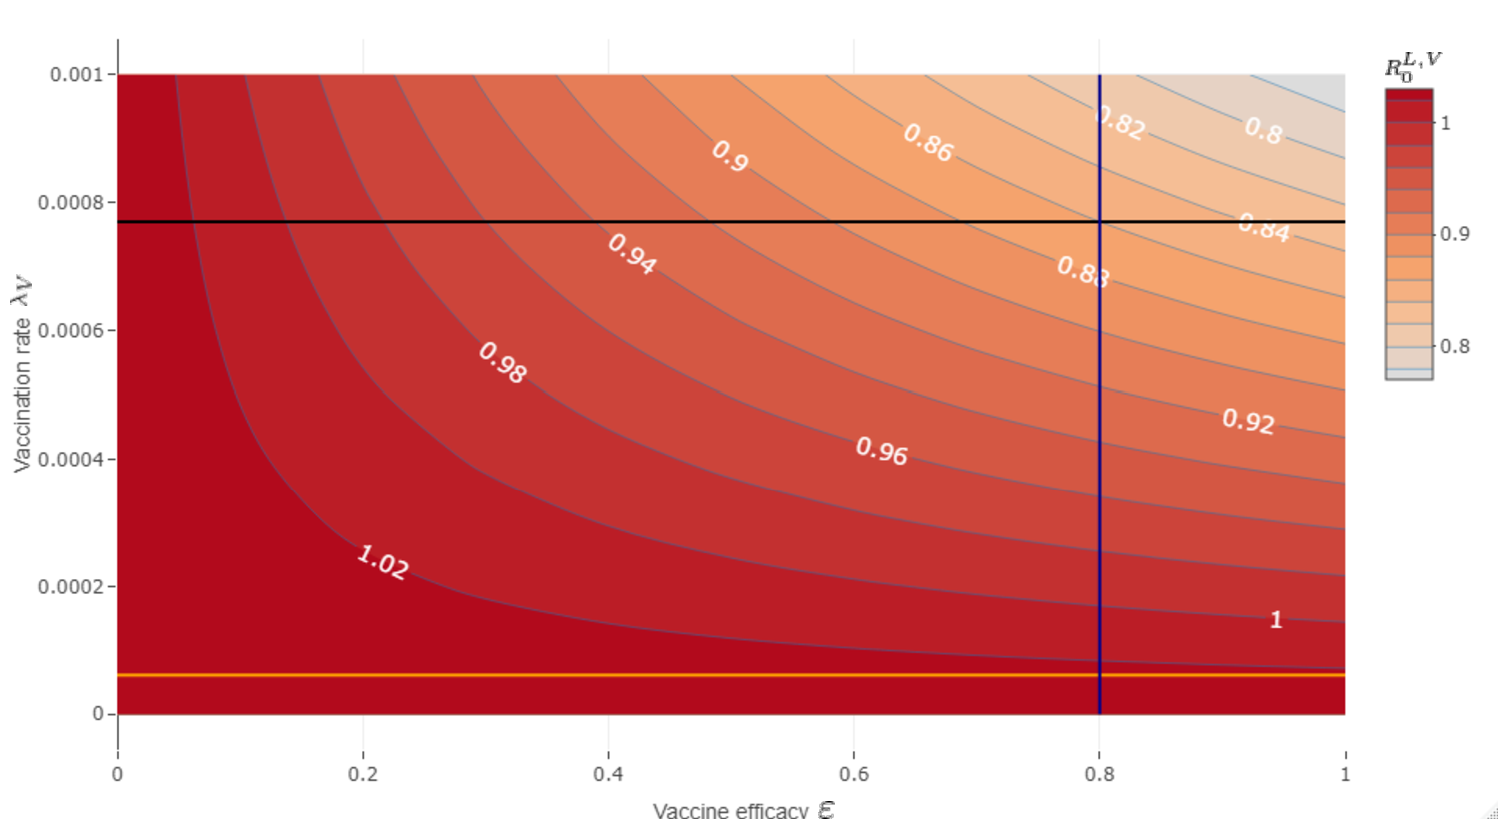
\includegraphics[scale=0.64,keepaspectratio]{./Figures/Rlv_contour.pdf}
    \caption{
        Contour plot of $R_0^{L,V}$ as a function of vaccine efficacy $(
        \varepsilon) $ and vaccination rate $(\lambda_V)$ and vaccine-induced
        immunity average time of one year. The solid orange line represents the
         value of $\lambda_{Vbase}=\num{0.0000611352}$,
        corresponding to a coverage $x_{coverage} = \num{0.2}$ and a horizon
        time $T=\num{365}$ days. The intersection of black line and blue line
        show a scenario in which it is possible to have the $R^{L, V}_0=0.86$,
        considering a vaccine efficacy of $\num{0.8}$ and a vaccination rate of
        $\num{0.0008}$.}
    \label{fig:rvcontour1}
\end{figure*}

\Cref{fig:rvcontour1} displays feasible combinations of vaccination rate and
vaccine
efficacy. In particular,  if we have chosen a vaccination rate below
$\num{0.00025}$
approximately, it is impossible to reduce to $R^{L,V}_0$ below one for any
vaccine
efficacy value. But, taking a vaccination rate greater than $\num{0.0004}$,
it is necessary a vaccine efficacy at least of \SI{50}{\percent} to have
$R^{L,V}_0 < 1$.
%
\begin{figure*}[tbh]
    \centering
    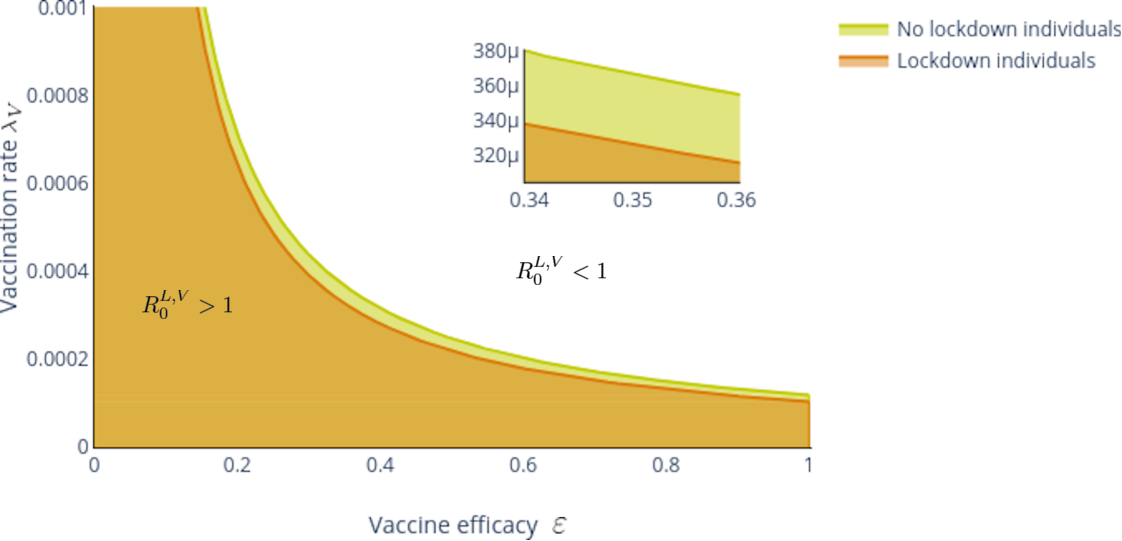
\includegraphics[scale=0.8,
    keepaspectratio]{./Figures/Rlv-feasible-region.pdf}
    \caption{
        Comparison of vaccination feasible region. The color regions show
        $R_0^{L,V}>1$, and white region $R_0^{L,V}<1$. Yellow-shaded region
        represent vaccination feasible region without lockdown individuals,
        orange-shaded region with lockdown individuals
        \href{https://plotly.com/~AdrianSalcedo/85/}{%
            https://plotly.com/~AdrianSalcedo/85/}
    }
    \label{fig:FeasibleRegion}
\end{figure*}
%
    We exhibit vaccination regions, with and without lockdown individuals in
\Cref{fig:FeasibleRegion}. Note that the region to have $R^{L,V}_0<1$ is
greater in the case with lockdown individuals than in the case without lockdown
individuals. For example, fixing a vaccine efficacy of $\num{0.35}$, we need to
vaccinate fewer individuals in the case of lockdown individuals than without
lockdown individuals to get $R^{L,V}_0<1$. And setting a vaccination rate of
$\num{0.00034}$, it is required at least a vaccine efficacy of $\num{0.35}$, in
case with lockdown individuals. But in the case without lockdown individuals, we
require at least $\num{0.36}$. These tell us that, implementing a strategy of
lockdown-vaccination instead of just vaccination reduces the number of
individuals to be vaccinated with less vaccine efficiency.

    \section{Optimal controlled version}
        \label{sec:optimal_controlled}
        %!TEX root = main.tex
Now we model vaccination, treatment, and lockdown as an optimal control problem.
According to dynamics in \Cref{eqn:base_dynamics}, we modulate lockdown
release and vaccination rates with time-dependent control signals
$u_L(t), u_V(t)$. We add acompartment $X_{vac}$ to count all the vaccine 
applications of lockdown, susceptible, exposed, asymptomatic, and recovered 
compartments. The following equation captures the dynamic of this process,
\begin{equation}
\label{eqn:counter}
  X'(t) =
    (\lambda_V + u_V(t))(L + S + E + I_A + R),
\end{equation}
and describes the number of applied vaccines at time $t$.
Let
$$
    x(t):= 
        (L, S, E, I_S, I_A, H, R, D, V, X_{vac}) ^ {\top}(t)
$$
the state of the system at time $t$. 
Thus we quantify the cost and reward of a vaccine
strategy policy via the penalization functional
\begin{equation}
    \label{eqn:cost_functional}
    \begin{aligned}
    J(u_L, u_V) := &
        \int _0 ^ T
            \underbrace{
                a_S p \kappa E(r) +
                a_H \delta_H I_s(r) +
                a_D
                \left[
                    \mu_{I_S} I_S(r) + \mu_H H(r)
                \right] 
            }_{DALY}
        dr
        \\
        & +
    \frac{1}{2}
        \int _0 ^ T
            \left[
                c_L u_L^2(r) +
                c_V u_v^2(r)
            \right]
        dr.
    \end{aligned}
\end{equation}
%
    In other words, we assume in functional $J$ that pandemic cost is 
proportional to the symptomatic hospitalized and death reported cases and that 
a vaccination and lockdown policies implies quadratic consumption of resources.
The quadratic form $q(u)=u^2$ of the cost is typical in economic
theory because the marginal cost\textemdash which is the derivative of the cost
$q$ when it exits\textemdash is assumed to be increasing. In the
vaccination context, consider $u_v=0.6$ and $u_v=0.05$; the change
in the cost from 60\% to 61\% is higher than that from 5\% to 6\%
of the population.

    Further, since we aim to simulate vaccination policies at different coverage
scenarios, we impose the vaccination counter state's final time condition
$X_{vac}(T)$
\begin{equation}
    \begin{aligned}
      x(T) &= 
        (
            \cdot, 
            \cdot, 
            \cdot, 
            \cdot, 
            \cdot, 
            \cdot, 
            \cdot, 
            \cdot, 
            \cdot, 
            \cdot,
        X_{vac }(T))^{\top}
      \in \Omega
      \\
      X_{vac}(T)
        &= x_{cover age},
      \\
      x_{coverage}
        & \in
        \left \{
          \text{Low(0.2)},\text{Mid(0.5)}, \text{High(0.8)}
        \right \},
    \end{aligned}
\end{equation}
%
where $\Omega$ is the positive invariant set
\begin{equation*}
    \begin{aligned}
        \Omega := 
            \Big \{
                x(t) ^{\top} \in [0,1]^{10}:
                L + S + E + I_S + I_A + H+ R + D + V = 1,
                \forall t \in [0, T]
            \Big \}.
    \end{aligned}
\end{equation*}
    Thus, given the time horizon $T$, we impose that the last fraction of
vaccinated populations corresponds to 20\%, 50\% or 80\%, and
the rest of final states as free. We also impose the path constraint
\begin{equation}
    \label{eqn:path_constrain}
    \Phi(x,t):= H(t) \leq B,
    \qquad \forall t \in [0, T],
\end{equation}
to ensure that healthcare services will not be overloaded. Here $\kappa$
denotes hospitalization rate, and $B$ is the load capacity of a
health system.

\begin{figure*}[tbh]
    \centering
        \includegraphics[scale=1.0, keepaspectratio]{%
        DiagramCOVID-19LockdownVaccinationModel.pdf}
    %

\tikzset{every picture/.style={line width=0.95pt}} %set default line width to 0.75pt        

\begin{tikzpicture}[x=0.75pt,y=0.75pt,yscale=-0.8,xscale=0.8]
%uncomment if require: \path (0,472); %set diagram left start at 0, and has height of 472

%Rounded Rect [id:dp9338258576556762] 
\draw   (131,159) .. controls (131,154.58) and (134.58,151) .. (139,151) -- (193,151) .. controls (197.42,151) and (201,154.58) .. (201,159) -- (201,183) .. controls (201,187.42) and (197.42,191) .. (193,191) -- (139,191) .. controls (134.58,191) and (131,187.42) .. (131,183) -- cycle ;
%Rounded Rect [id:dp03550846434827437] 
\draw   (252,159) .. controls (252,154.58) and (255.58,151) .. (260,151) -- (314,151) .. controls (318.42,151) and (322,154.58) .. (322,159) -- (322,183) .. controls (322,187.42) and (318.42,191) .. (314,191) -- (260,191) .. controls (255.58,191) and (252,187.42) .. (252,183) -- cycle ;
%Rounded Rect [id:dp2096597210016533] 
\draw   (391.5,99) .. controls (391.5,94.58) and (395.08,91) .. (399.5,91) -- (453.5,91) .. controls (457.92,91) and (461.5,94.58) .. (461.5,99) -- (461.5,123) .. controls (461.5,127.42) and (457.92,131) .. (453.5,131) -- (399.5,131) .. controls (395.08,131) and (391.5,127.42) .. (391.5,123) -- cycle ;
%Rounded Rect [id:dp4192775592826552] 
\draw   (391.5,219.5) .. controls (391.5,215.08) and (395.08,211.5) .. (399.5,211.5) -- (453.5,211.5) .. controls (457.92,211.5) and (461.5,215.08) .. (461.5,219.5) -- (461.5,243.5) .. controls (461.5,247.92) and (457.92,251.5) .. (453.5,251.5) -- (399.5,251.5) .. controls (395.08,251.5) and (391.5,247.92) .. (391.5,243.5) -- cycle ;
%Rounded Rect [id:dp9412674774350195] 
\draw   (671.5,219.5) .. controls (671.5,215.08) and (675.08,211.5) .. (679.5,211.5) -- (733.5,211.5) .. controls (737.92,211.5) and (741.5,215.08) .. (741.5,219.5) -- (741.5,243.5) .. controls (741.5,247.92) and (737.92,251.5) .. (733.5,251.5) -- (679.5,251.5) .. controls (675.08,251.5) and (671.5,247.92) .. (671.5,243.5) -- cycle ;
%Rounded Rect [id:dp7750331540351684] 
\draw   (531,309.33) .. controls (531,304.92) and (534.58,301.33) .. (539,301.33) -- (593,301.33) .. controls (597.42,301.33) and (601,304.92) .. (601,309.33) -- (601,333.33) .. controls (601,337.75) and (597.42,341.33) .. (593,341.33) -- (539,341.33) .. controls (534.58,341.33) and (531,337.75) .. (531,333.33) -- cycle ;
%Rounded Rect [id:dp22729858034129236] 
\draw   (531,220) .. controls (531,215.58) and (534.58,212) .. (539,212) -- (593,212) .. controls (597.42,212) and (601,215.58) .. (601,220) -- (601,244) .. controls (601,248.42) and (597.42,252) .. (593,252) -- (539,252) .. controls (534.58,252) and (531,248.42) .. (531,244) -- cycle ;
%Straight Lines [id:da8056305543799926] 
\draw    (201.33,162.17) -- (249.67,162.01) ;
\draw [shift={(251.67,162)}, rotate = 539.81] [color={rgb, 255:red, 0; green, 0; blue, 0 }  ][line width=0.75]    (10.93,-3.29) .. controls (6.95,-1.4) and (3.31,-0.3) .. (0,0) .. controls (3.31,0.3) and (6.95,1.4) .. (10.93,3.29)   ;
%Straight Lines [id:da2787683579538649] 
\draw    (322.78,171.33) -- (357.67,171.17) ;
%Straight Lines [id:da21916666537860907] 
\draw    (357.67,111.17) -- (389.67,111.32) ;
\draw [shift={(391.67,111.33)}, rotate = 180.28] [color={rgb, 255:red, 0; green, 0; blue, 0 }  ][line width=0.75]    (10.93,-3.29) .. controls (6.95,-1.4) and (3.31,-0.3) .. (0,0) .. controls (3.31,0.3) and (6.95,1.4) .. (10.93,3.29)   ;
%Straight Lines [id:da8438200798129222] 
\draw    (357.67,110.6) -- (357.67,231.17) ;
%Straight Lines [id:da7337155371803761] 
\draw    (357.67,231.17) -- (389.67,231.32) ;
\draw [shift={(391.67,231.33)}, rotate = 180.28] [color={rgb, 255:red, 0; green, 0; blue, 0 }  ][line width=0.75]    (10.93,-3.29) .. controls (6.95,-1.4) and (3.31,-0.3) .. (0,0) .. controls (3.31,0.3) and (6.95,1.4) .. (10.93,3.29)   ;
%Straight Lines [id:da509274682669141] 
\draw    (461.43,226) -- (516.2,226.39) -- (529.2,226.49) ;
\draw [shift={(531.2,226.5)}, rotate = 180.41] [color={rgb, 255:red, 0; green, 0; blue, 0 }  ][line width=0.75]    (10.93,-3.29) .. controls (6.95,-1.4) and (3.31,-0.3) .. (0,0) .. controls (3.31,0.3) and (6.95,1.4) .. (10.93,3.29)   ;
%Straight Lines [id:da3183759306298827] 
\draw    (500.63,321.73) -- (529,321.36) ;
\draw [shift={(531,321.33)}, rotate = 539.25] [color={rgb, 255:red, 0; green, 0; blue, 0 }  ][line width=0.75]    (10.93,-3.29) .. controls (6.95,-1.4) and (3.31,-0.3) .. (0,0) .. controls (3.31,0.3) and (6.95,1.4) .. (10.93,3.29)   ;
%Straight Lines [id:da6861028849351065] 
\draw    (462,236) -- (500.88,235.98) ;
%Straight Lines [id:da9190171216881116] 
\draw    (500.88,235.98) -- (500.63,321.73) ;
%Straight Lines [id:da03313994658252273] 
\draw    (600.33,241.33) -- (657.2,241.39) -- (669,241.27) ;
\draw [shift={(671,241.25)}, rotate = 539.4100000000001] [color={rgb, 255:red, 0; green, 0; blue, 0 }  ][line width=0.75]    (10.93,-3.29) .. controls (6.95,-1.4) and (3.31,-0.3) .. (0,0) .. controls (3.31,0.3) and (6.95,1.4) .. (10.93,3.29)   ;
%Straight Lines [id:da6934604539767528] 
\draw    (566.33,252) -- (566.65,298.92) ;
\draw [shift={(566.67,300.92)}, rotate = 269.61] [color={rgb, 255:red, 0; green, 0; blue, 0 }  ][line width=0.75]    (10.93,-3.29) .. controls (6.95,-1.4) and (3.31,-0.3) .. (0,0) .. controls (3.31,0.3) and (6.95,1.4) .. (10.93,3.29)   ;
%Straight Lines [id:da6916456040068684] 
\draw    (461,111.17) -- (706.6,112) ;
%Straight Lines [id:da7246498566982733] 
\draw    (706.6,112) -- (707.32,209.17) ;
\draw [shift={(707.33,211.17)}, rotate = 269.58] [color={rgb, 255:red, 0; green, 0; blue, 0 }  ][line width=0.75]    (10.93,-3.29) .. controls (6.95,-1.4) and (3.31,-0.3) .. (0,0) .. controls (3.31,0.3) and (6.95,1.4) .. (10.93,3.29)   ;
%Straight Lines [id:da5396778112959429] 
\draw    (427,161.17) -- (427,211.5) ;
%Straight Lines [id:da7180507787496266] 
\draw    (424.7,160.93) -- (621.3,161.32) ;
%Straight Lines [id:da3365589163505732] 
\draw    (621,221.35) -- (669.13,221.35) ;
\draw [shift={(671.13,221.35)}, rotate = 180] [color={rgb, 255:red, 0; green, 0; blue, 0 }  ][line width=0.75]    (10.93,-3.29) .. controls (6.95,-1.4) and (3.31,-0.3) .. (0,0) .. controls (3.31,0.3) and (6.95,1.4) .. (10.93,3.29)   ;
%Straight Lines [id:da7818385183529692] 
\draw    (620.8,161.2) -- (621,221.35) ;
%Straight Lines [id:da20994732667721105] 
\draw [color={rgb, 255:red, 245; green, 166; blue, 35 }  ,draw opacity=1 ][fill={rgb, 255:red, 65; green, 117; blue, 5 }  ,fill opacity=1 ]   (101.15,170.97) -- (128.54,171.26) ;
\draw [shift={(130.54,171.28)}, rotate = 180.6] [color={rgb, 255:red, 245; green, 166; blue, 35 }  ,draw opacity=1 ][line width=0.75]    (10.93,-3.29) .. controls (6.95,-1.4) and (3.31,-0.3) .. (0,0) .. controls (3.31,0.3) and (6.95,1.4) .. (10.93,3.29)   ;
%Straight Lines [id:da9409632697808414] 
\draw [color={rgb, 255:red, 65; green, 117; blue, 5 }  ,draw opacity=1 ]   (130.75,181.29) -- (103,181.36) ;
\draw [shift={(101,181.37)}, rotate = 359.86] [color={rgb, 255:red, 65; green, 117; blue, 5 }  ,draw opacity=1 ][line width=0.75]    (10.93,-3.29) .. controls (6.95,-1.4) and (3.31,-0.3) .. (0,0) .. controls (3.31,0.3) and (6.95,1.4) .. (10.93,3.29)   ;
%Straight Lines [id:da671739616587531] 
\draw [color={rgb, 255:red, 65; green, 117; blue, 5 }  ,draw opacity=1 ]   (286.82,190.79) -- (286.82,218.85) ;
\draw [shift={(286.82,220.85)}, rotate = 270] [color={rgb, 255:red, 65; green, 117; blue, 5 }  ,draw opacity=1 ][line width=0.75]    (10.93,-3.29) .. controls (6.95,-1.4) and (3.31,-0.3) .. (0,0) .. controls (3.31,0.3) and (6.95,1.4) .. (10.93,3.29)   ;
%Straight Lines [id:da4612478738976049] 
\draw [color={rgb, 255:red, 65; green, 117; blue, 5 }  ,draw opacity=1 ]   (427.25,251.79) -- (427.48,279.54) ;
\draw [shift={(427.5,281.54)}, rotate = 269.52] [color={rgb, 255:red, 65; green, 117; blue, 5 }  ,draw opacity=1 ][line width=0.75]    (10.93,-3.29) .. controls (6.95,-1.4) and (3.31,-0.3) .. (0,0) .. controls (3.31,0.3) and (6.95,1.4) .. (10.93,3.29)   ;
%Straight Lines [id:da6463966696699537] 
\draw [color={rgb, 255:red, 65; green, 117; blue, 5 }  ,draw opacity=1 ]   (427.5,92.04) -- (427.19,63.25) ;
\draw [shift={(427.17,61.25)}, rotate = 449.38] [color={rgb, 255:red, 65; green, 117; blue, 5 }  ,draw opacity=1 ][line width=0.75]    (10.93,-3.29) .. controls (6.95,-1.4) and (3.31,-0.3) .. (0,0) .. controls (3.31,0.3) and (6.95,1.4) .. (10.93,3.29)   ;
%Straight Lines [id:da5390055225547872] 
\draw [color={rgb, 255:red, 65; green, 117; blue, 5 }  ,draw opacity=1 ]   (567.25,211.92) -- (567.02,182.67) ;
\draw [shift={(567,180.67)}, rotate = 449.54] [color={rgb, 255:red, 65; green, 117; blue, 5 }  ,draw opacity=1 ][line width=0.75]    (10.93,-3.29) .. controls (6.95,-1.4) and (3.31,-0.3) .. (0,0) .. controls (3.31,0.3) and (6.95,1.4) .. (10.93,3.29)   ;
%Straight Lines [id:da5965287355289506] 
\draw [color={rgb, 255:red, 65; green, 117; blue, 5 }  ,draw opacity=1 ]   (742,231.29) -- (768.88,231.23) ;
\draw [shift={(770.88,231.23)}, rotate = 539.88] [color={rgb, 255:red, 65; green, 117; blue, 5 }  ,draw opacity=1 ][line width=0.75]    (10.93,-3.29) .. controls (6.95,-1.4) and (3.31,-0.3) .. (0,0) .. controls (3.31,0.3) and (6.95,1.4) .. (10.93,3.29)   ;
%Straight Lines [id:da8186275398290976] 
\draw [color={rgb, 255:red, 245; green, 166; blue, 35 }  ,draw opacity=1 ]   (212.25,345.21) -- (240,345.17) ;
\draw [shift={(242,345.17)}, rotate = 539.9200000000001] [color={rgb, 255:red, 245; green, 166; blue, 35 }  ,draw opacity=1 ][line width=0.75]    (10.93,-3.29) .. controls (6.95,-1.4) and (3.31,-0.3) .. (0,0) .. controls (3.31,0.3) and (6.95,1.4) .. (10.93,3.29)   ;
%Straight Lines [id:da2473783506649132] 
\draw [color={rgb, 255:red, 65; green, 117; blue, 5 }  ,draw opacity=1 ]   (241.75,365.46) -- (214.25,365.46) ;
\draw [shift={(212.25,365.46)}, rotate = 360] [color={rgb, 255:red, 65; green, 117; blue, 5 }  ,draw opacity=1 ][line width=0.75]    (10.93,-3.29) .. controls (6.95,-1.4) and (3.31,-0.3) .. (0,0) .. controls (3.31,0.3) and (6.95,1.4) .. (10.93,3.29)   ;
%Rounded Rect [id:dp8809691932687975] 
\draw  [fill={rgb, 255:red, 248; green, 231; blue, 28 }  ,fill opacity=1 ] (131,259) .. controls (131,254.58) and (134.58,251) .. (139,251) -- (193,251) .. controls (197.42,251) and (201,254.58) .. (201,259) -- (201,283) .. controls (201,287.42) and (197.42,291) .. (193,291) -- (139,291) .. controls (134.58,291) and (131,287.42) .. (131,283) -- cycle ;
%Rounded Rect [id:dp20452328105731965] 
\draw  [fill={rgb, 255:red, 248; green, 231; blue, 28 }  ,fill opacity=1 ] (131,59) .. controls (131,54.58) and (134.58,51) .. (139,51) -- (193,51) .. controls (197.42,51) and (201,54.58) .. (201,59) -- (201,83) .. controls (201,87.42) and (197.42,91) .. (193,91) -- (139,91) .. controls (134.58,91) and (131,87.42) .. (131,83) -- cycle ;
%Straight Lines [id:da7332016409842015] 
\draw    (230.56,180.67) -- (249.67,180.67) ;
\draw [shift={(251.67,180.67)}, rotate = 180] [color={rgb, 255:red, 0; green, 0; blue, 0 }  ][line width=0.75]    (10.93,-3.29) .. controls (6.95,-1.4) and (3.31,-0.3) .. (0,0) .. controls (3.31,0.3) and (6.95,1.4) .. (10.93,3.29)   ;
%Straight Lines [id:da9863388911939545] 
\draw    (230.56,180.67) -- (231.44,270.89) ;
%Straight Lines [id:da8080535215203265] 
\draw    (201.25,271.35) -- (231.44,270.89) ;
%Straight Lines [id:da40743845785244703] 
\draw    (166.11,250.89) -- (166.33,193.78) ;
\draw [shift={(166.33,191.78)}, rotate = 450.22] [color={rgb, 255:red, 0; green, 0; blue, 0 }  ][line width=0.75]    (10.93,-3.29) .. controls (6.95,-1.4) and (3.31,-0.3) .. (0,0) .. controls (3.31,0.3) and (6.95,1.4) .. (10.93,3.29)   ;
%Straight Lines [id:da9322929691633284] 
\draw    (101.2,161.37) -- (128.78,161.21) ;
\draw [shift={(130.78,161.19)}, rotate = 539.6700000000001] [color={rgb, 255:red, 0; green, 0; blue, 0 }  ][line width=0.75]    (10.93,-3.29) .. controls (6.95,-1.4) and (3.31,-0.3) .. (0,0) .. controls (3.31,0.3) and (6.95,1.4) .. (10.93,3.29)   ;
%Straight Lines [id:da39718296722033697] 
\draw    (181.22,151) -- (181.44,91.89) ;
\draw [shift={(181.44,89.89)}, rotate = 450.21] [color={rgb, 255:red, 0; green, 0; blue, 0 }  ][line width=0.75]    (10.93,-3.29) .. controls (6.95,-1.4) and (3.31,-0.3) .. (0,0) .. controls (3.31,0.3) and (6.95,1.4) .. (10.93,3.29)   ;
%Straight Lines [id:da5809696066442677] 
\draw    (151.56,90.89) -- (151.66,149.11) ;
\draw [shift={(151.67,151.11)}, rotate = 269.89] [color={rgb, 255:red, 0; green, 0; blue, 0 }  ][line width=0.75]    (10.93,-3.29) .. controls (6.95,-1.4) and (3.31,-0.3) .. (0,0) .. controls (3.31,0.3) and (6.95,1.4) .. (10.93,3.29)   ;
%Straight Lines [id:da793642305015831] 
\draw [color={rgb, 255:red, 65; green, 117; blue, 5 }  ,draw opacity=1 ]   (166,50.54) -- (166.16,23.08) ;
\draw [shift={(166.17,21.08)}, rotate = 450.32] [color={rgb, 255:red, 65; green, 117; blue, 5 }  ,draw opacity=1 ][line width=0.75]    (10.93,-3.29) .. controls (6.95,-1.4) and (3.31,-0.3) .. (0,0) .. controls (3.31,0.3) and (6.95,1.4) .. (10.93,3.29)   ;
%Straight Lines [id:da6558914162483227] 
\draw    (61.18,71.03) -- (128.8,70.68) ;
\draw [shift={(130.8,70.67)}, rotate = 539.7] [color={rgb, 255:red, 0; green, 0; blue, 0 }  ][line width=0.75]    (10.93,-3.29) .. controls (6.95,-1.4) and (3.31,-0.3) .. (0,0) .. controls (3.31,0.3) and (6.95,1.4) .. (10.93,3.29)   ;
%Straight Lines [id:da352457903437118] 
\draw    (61.18,71.03) -- (61.36,321.21) ;
%Straight Lines [id:da6614557049237877] 
\draw    (166,291.3) -- (165.91,321.21) ;
%Straight Lines [id:da33095535888136296] 
\draw    (61.36,321.21) -- (165.91,321.21) ;
%Straight Lines [id:da269007580963348] 
\draw    (201.64,71.03) -- (286.45,71.21) ;
%Straight Lines [id:da3843881794607171] 
\draw    (286.45,71.21) -- (285.92,149.39) ;
\draw [shift={(285.91,151.39)}, rotate = 270.39] [color={rgb, 255:red, 0; green, 0; blue, 0 }  ][line width=0.75]    (10.93,-3.29) .. controls (6.95,-1.4) and (3.31,-0.3) .. (0,0) .. controls (3.31,0.3) and (6.95,1.4) .. (10.93,3.29)   ;
%Straight Lines [id:da5569228544903815] 
\draw [color={rgb, 255:red, 74; green, 144; blue, 226 }  ,draw opacity=1 ][fill={rgb, 255:red, 65; green, 117; blue, 5 }  ,fill opacity=1 ]   (101.15,260.97) -- (128.54,261.26) ;
\draw [shift={(130.54,261.28)}, rotate = 180.6] [color={rgb, 255:red, 74; green, 144; blue, 226 }  ,draw opacity=1 ][line width=0.75]    (10.93,-3.29) .. controls (6.95,-1.4) and (3.31,-0.3) .. (0,0) .. controls (3.31,0.3) and (6.95,1.4) .. (10.93,3.29)   ;
%Straight Lines [id:da8309131427834217] 
\draw [color={rgb, 255:red, 65; green, 117; blue, 5 }  ,draw opacity=1 ]   (130.75,281.29) -- (103,281.36) ;
\draw [shift={(101,281.37)}, rotate = 359.86] [color={rgb, 255:red, 65; green, 117; blue, 5 }  ,draw opacity=1 ][line width=0.75]    (10.93,-3.29) .. controls (6.95,-1.4) and (3.31,-0.3) .. (0,0) .. controls (3.31,0.3) and (6.95,1.4) .. (10.93,3.29)   ;
%Straight Lines [id:da0682900101015288] 
\draw [color={rgb, 255:red, 74; green, 144; blue, 226 }  ,draw opacity=1 ][fill={rgb, 255:red, 65; green, 117; blue, 5 }  ,fill opacity=1 ]   (213.35,326.17) -- (240.74,326.46) ;
\draw [shift={(242.74,326.48)}, rotate = 180.6] [color={rgb, 255:red, 74; green, 144; blue, 226 }  ,draw opacity=1 ][line width=0.75]    (10.93,-3.29) .. controls (6.95,-1.4) and (3.31,-0.3) .. (0,0) .. controls (3.31,0.3) and (6.95,1.4) .. (10.93,3.29)   ;

% Text Node
\draw (161,163) node [anchor=north west][inner sep=0.75pt]   [align=left] {$\displaystyle S$};
% Text Node
\draw (281.33,163.33) node [anchor=north west][inner sep=0.75pt]   [align=left] {$\displaystyle E$};
% Text Node
\draw (418.67,102) node [anchor=north west][inner sep=0.75pt]   [align=left] {$\displaystyle I_{A}$};
% Text Node
\draw (420.33,223.33) node [anchor=north west][inner sep=0.75pt]   [align=left] {$\displaystyle I_{S}$};
% Text Node
\draw (558.33,223) node [anchor=north west][inner sep=0.75pt]   [align=left] {$\displaystyle H$};
% Text Node
\draw (701.33,222.33) node [anchor=north west][inner sep=0.75pt]   [align=left] {$\displaystyle R$};
% Text Node
\draw (559.67,312.67) node [anchor=north west][inner sep=0.75pt]   [align=left] {$\displaystyle D$};
% Text Node
\draw (244,355.17) node [anchor=north west][inner sep=0.75pt]   [align=left] {$\displaystyle :\mu $};
% Text Node
\draw (244.33,332) node [anchor=north west][inner sep=0.75pt]   [align=left] {$\displaystyle :( 1-\theta ) \mu N^{*}$};
% Text Node
\draw (215.5,140.67) node [anchor=north west][inner sep=0.75pt]   [align=left] {$\displaystyle \lambda $};
% Text Node
\draw (358.5,232.5) node [anchor=north west][inner sep=0.75pt]   [align=left] {$\displaystyle p\kappa $};
% Text Node
\draw (327,85) node [anchor=north west][inner sep=0.75pt]   [align=left] {$\displaystyle ( 1-p) \kappa $};
% Text Node
\draw (593,85) node [anchor=north west][inner sep=0.75pt]   [align=left] {$\displaystyle \gamma _{A}$};
% Text Node
\draw (532,134.5) node [anchor=north west][inner sep=0.75pt]   [align=left] {$\displaystyle \gamma _{S}$};
% Text Node
\draw (486.5,202.5) node [anchor=north west][inner sep=0.75pt]   [align=left] {$\displaystyle \delta _{H}$};
% Text Node
\draw (579,263) node [anchor=north west][inner sep=0.75pt]   [align=left] {$\displaystyle \mu _{H}$};
% Text Node
\draw (620.5,239) node [anchor=north west][inner sep=0.75pt]   [align=left] {$ $$\displaystyle \gamma _{H}$};
% Text Node
\draw (470.5,273.5) node [anchor=north west][inner sep=0.75pt]   [align=left] {$\displaystyle \mu _{I_{S}}$};
% Text Node
\draw (160,262) node [anchor=north west][inner sep=0.75pt]   [align=left] {$\displaystyle L$};
% Text Node
\draw (159.2,62) node [anchor=north west][inner sep=0.75pt]   [align=left] {$\displaystyle V$};
% Text Node
\draw (185.17,108) node [anchor=north west][inner sep=0.75pt]   [align=left] {$\displaystyle \textcolor[rgb]{0.82,0.01,0.11}{\lambda }\textcolor[rgb]{0.82,0.01,0.11}{_{V}} +\textcolor[rgb]{0.29,0.56,0.89}{u}\textcolor[rgb]{0.29,0.56,0.89}{_{V}}\textcolor[rgb]{0.29,0.56,0.89}{(}\textcolor[rgb]{0.29,0.56,0.89}{t}\textcolor[rgb]{0.29,0.56,0.89}{)}$};
% Text Node
\draw (86.17,213.33) node [anchor=north west][inner sep=0.75pt]   [align=left] {$\displaystyle \textcolor[rgb]{0.82,0.01,0.11}{\delta }\textcolor[rgb]{0.82,0.01,0.11}{_{L}} +\textcolor[rgb]{0.29,0.56,0.89}{u}\textcolor[rgb]{0.29,0.56,0.89}{_{L}}\textcolor[rgb]{0.29,0.56,0.89}{(}\textcolor[rgb]{0.29,0.56,0.89}{t}\textcolor[rgb]{0.29,0.56,0.89}{)}$};
% Text Node
\draw (28.17,192) node [anchor=north west][inner sep=0.75pt]   [align=left] {$\displaystyle \textcolor[rgb]{0,0,0}{\lambda }\textcolor[rgb]{0,0,0}{_{V}}$};
% Text Node
\draw (237.17,49) node [anchor=north west][inner sep=0.75pt]   [align=left] {$\displaystyle \textcolor[rgb]{0,0,0}{\lambda }\textcolor[rgb]{0,0,0}{(}\textcolor[rgb]{0,0,0}{1-\epsilon }\textcolor[rgb]{0,0,0}{)}$};
% Text Node
\draw (238.17,226) node [anchor=north west][inner sep=0.75pt]   [align=left] {$\displaystyle \textcolor[rgb]{0,0,0}{\epsilon \lambda }$};
% Text Node
\draw (213,385) node [anchor=north west][inner sep=0.75pt]   [align=left] {$\displaystyle  \begin{array}{{>{\displaystyle}l}}
\min_{u\in \mathcal{U}} \ J( u_{L} ,u_{V})\\
X_{vacc}( T) \ =\ x_{coverage}\\
\phi ( x,t) :=\kappa \ I_{S}( t) \leq B,\ \forall \ t\ \in [ 0,T]
\end{array}$};
% Text Node
\draw (244.6,313.27) node [anchor=north west][inner sep=0.75pt]   [align=left] {$\displaystyle :\theta \mu N^{*}$};


\end{tikzpicture}

    \caption{
        Compartmental diagram of COVID-19 transmission dynamics that includes
        optimal vaccination dynamics, penalization and a path constraint
    }
    \label{fig:DiagramControl}
\end{figure*}

    Given a fixed time horizon and vaccine efficacy,
we estimate nominal lockdown-vaccination rates by 
\begin{equation}
    \begin{aligned}
        x^L_{release} &= L(0)(1 - \exp(-\delta_L T))
        \\
        x^V_{coverage} &= 1 - \exp(-\lambda_V T) .      
    \end{aligned}
\end{equation}
    That is, $(\delta_L, \lambda_V)^{\top}$ respectively denotes, 
the constant rate to cover and release fractions 
$(x^L_{release}, x_{coverage} ^ V)^{\top}$ in time horizon $T$.
Thus, according to these rates, we postulate a policy $(u_L, u_V)^{\top}$ that
modulates lockdown-vaccination rates according to 
$\delta_L$ and  $\lambda_V$ as a baseline. Then,
optimal lockdown-vaccination amplifies or attenuates the estimated baseline
$\delta_L$, $\lambda_V$ in the square
$\textbf{}
    [\delta_L ^ {\min}, \delta_L ^ {\max}] \times
    [\lambda_V ^ {\min}, \lambda_V ^ {\max}]
\textbf{}$
to optimize functional $J(\cdot)$\textemdash minimizing
symptomatic, death reported cases and optimizing resources.

    We aim to minimize the cost functional
\eqref{eqn:cost_functional}\textemdash over an appropriated functional
space\textemdash subject to the dynamics in
\cref{eqn:base_dynamics,eqn:counter}, boundary conditions, and the path
constraint in \eqref{eqn:path_constrain}.
That is, we look for lockdown-vaccination policies 
$\mathbf{u}:=(u_L(\cdot), u_V(\cdot))$, which solve the following optimal
control problem (OCP)
\begin{equation}
    \label{eqn:lockdown_vaccination_ocp}
    \begin{aligned}
        \min_{\mathbf{u} \in \mathcal{U}}
            J(u_L, u_V) := &
                \int_0 ^  T
                    a_S p \kappa E(r) +
                    a_H \delta_H I_s(r) +
                    a_D
                    \left[
                        \mu_{I_S} I_S(r) + \mu_H H(r)
                    \right]
                dr +
        \\
                &
                \int_0^T
                    \frac{1}{2}
                    \left[
                        c_L u_L^2(r) +
                        c_V u_v^2(r)
                    \right]
                    dr.
        \\
            \text{s. t.} &
        \\
            L' & =  \theta \mu N^{\star}
                -\epsilon \lambda L - (u_L(t) + \delta_L) L - \mu L
        \\
            S' & =
                (1 - \theta) \mu N^\star
                + (u_L(t) + \delta_L) L
                + \delta_V V
                + \delta_R R
        \\
                & \qquad -
                \left[
                \lambda + (\lambda_V + u_V(t)) + \mu
                \right] S
        \\
            E' &=
                \lambda (\epsilon L + (1-\varepsilon) V + S)
                - (\kappa + \mu) E
        \\
            I_S' &=
                p \kappa E
                % + (1 - q) \gamma_M M(t)
                - (\gamma_S +
                    \mu_{I_S} +
                    \delta_H +
                    %u_M(t) +
                    \mu) I_S
        \\
            I_A' &=
                (1 - p) \kappa E - (\gamma_A + \mu) I_A
        \\
            H' &=
                \delta_H I_S - (\gamma_H + \mu_H + \mu) H
        \\
            R'  &=
                \gamma_S I_S +
                \gamma_A I_A +
                \gamma_H H % +
                - (\delta_R + \mu) R
        \\
            D' &=
                \mu_{I_S} I_S + \mu_H H
        \\
            V' &=
                (\lambda_V + u_V(t)) S
                - \left[
                (1 - \varepsilon) \lambda
                + \delta_V
                + \mu
                \right ] V
        \\
        \\
            \frac{dX_{vac}}{dt}
                &=
                (u_V(t) + \lambda_V)
                \left[
                    L + S + E + I_A + R
                \right]
        \\
            \frac{d Y_{I_S}}{dt}
                & = p \kappa E
        \\
            \lambda &:=
                \frac{\beta_A I_A + \beta_S I_S}{N^{\star}}
        \\
        \\
            L(0) &= L_0,
            \ S(0) = S_0,
            \ E(0) = E_0,
            \ I_S(0) = I_{S_{0}},
      \\
            I_A(0) &= I_{A_{0}},
            H(0) = H_0, \
            \ R(0) = R_0, \ D(0) = D_0,
      \\
            V(0) &= 0, \ X_{vac}(0) = 0, \quad
            u_V(.) \in [u_{\min}, u^{\max}],
      \\
            X_{vac}(T) &= x_{coverage},
      \quad
            \kappa I_S(t) \leq B, \qquad
            \forall t \in [0, T],
      \\
            N^{\star}(t) &=
                L + S +E + I_S + I_A +
                H + R + V
        \end{aligned}
\end{equation}

    \section{Numerical Experiments}
        \label{sec:numerical_experiments}
        %!TEX root = main.tex
\subsection{Methodology}
    We simulate a scenario corresponding to a hypothetical but plausible initial conditions and parameters. We integrate model in
\Cref{eqn:lockdown_vaccination_ocp} by classic Runge Kutta scheme and solve the
optimization stage with the so-called Differntial Evolution method.
Differential Evolution (DE) \cite{Storn1997} is an evolutionary
algorithm successfully employed for global optimization
\cite{Bilal2020}. The method is designed to optimize functions
$f:\mathbb{R}^n \to \mathbb{R}$. Nevertheless, DE can be applied to
optimize a functional as stated in \cite{CANTUNetAl}. The method can be
coded following Algorithm \ref{alg:DE1}, where an initial random
population on the search space $\mathcal{V}$ of size $N_p$ is subjected
to mutation, crossover and selection. After this process a new
population is created which, again would be subjected to the
evolutionary process. This process is repeated until some stopping
criteria is fulfilled. Finally the best individual (according to some
objective function $f_{ob}$ to optimize) is extracted. These operations
are conducted by the operators $\mathbf{X}_0$, $\mathbf{M}$,
$\mathbf{C}$, $\mathbf{S}$, $\mathbf{x}_{best}$;  whose explicit form
are coded in \cite{Penunuri2016}.

In the optimization of this study,
the mutation scale factor $F$ and the crossover probability $C_r$ were
taken as 1 and 0.3 respectively, additional $N_p$ has been taken as 4
times the number of parameters (the dimension of the vector used to
describe the two controls\textemdash see \cite{CANTUNetAl}), which in our case was
of 180. As stopping criteria we have used a maximum number of
generations which is taken as \num{5000}.

    We provide in \cite{gitHub_b} a GitHub repository with all regarding R
and Fortran sources for the sake of reproductivity. This repository also
encloses data sources and a Wolfrang Mathematica notebook to reproduce all
reported figures.
%
%
\begin{algorithm}[htb]
  \caption{Differential Evolution Algorithm}
  \label{alg:DE1}
  \begin{algorithmic}
    % \small
    \State $X \leftarrow \mathbf{X}_0(Np,\mathcal{V})$
    \While{(the stopping criterion has not been met)}
    \State $M \leftarrow \mathbf{M}(X,F,\mathcal{V})$
    \State $C \leftarrow \mathbf{C}(X,M,C_r)$
    \State $X \leftarrow \mathbf{S}(X,C,f_{ob})$
    \EndWhile
    \State $\mathbf{x}_{best} \leftarrow \mathbf{Best}(X, f_{ob})$
  \end{algorithmic}
\end{algorithm}

        %!TEX root = main.tex
%Vaccine development
\begin{figure*}
    \centering
    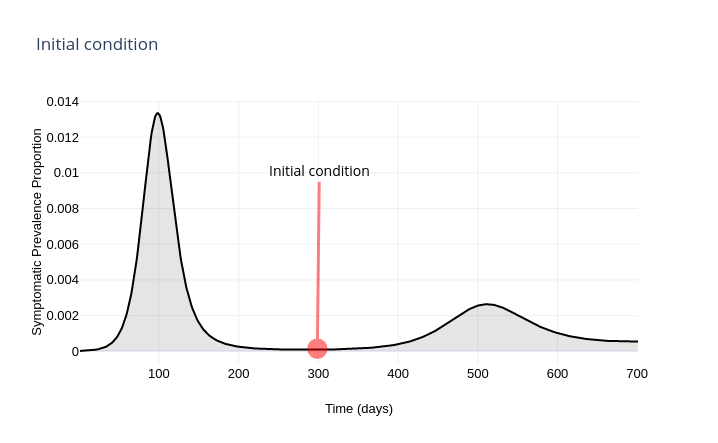
\includegraphics[scale=0.5, keepaspectratio]{figs/InitialCondition}
    \caption[Initial condition]{
        Initial condition scheme. We assume a positive prevalence. 
        For reference, at the date of write this manuscript, prevalence in CDMX 
        is around \SI{16000}{cases}, see
        \href{https://plotly.com/~sauld/36/}{https://plotly.com/~sauld/36/}
        to display an electronic viewer.}
        \label{fig:initialcondition}
\end{figure*}
\subsection{Simulation}
 According to official Governmental communication in December, Mexico treated  
\num{36000000} doses  Pfizer-Biotech, \num{76000000} doses with Aztra Seneca 
\num{18000000} quantities of Cansino-BIO. Other developments 
also are running the third Phase, and with high probability,  in the third
quarter of 2021, some of these developments will incorporate into Mexico's 
vaccine portfolio. Despite official agreements, each vaccine's delivery schedule 
is under uncertainty and-or subject to the approval of COFEPRIS.

The first accepted vaccine\textemdash Pfizer-BioNTech's BNT162b2\textemdash has 
an efficacy above \SI{90}{\percent} and requires two doses to achieve immunity. 
The other mentioned developments have a very similar profile but require 
different logistic management and stock allocation.
Thus, we face designing a dose application schedule subject to a given vaccine 
stock applied in a given period. To this end, we solve the optimal control 
problem \eqref{eqn:lockdown_vaccination_ocp}. 
We understand as solution of this problem a pair $(x(\cdot), u(\cdot))$ where
\begin{equation}
    \begin{aligned}
        x(t) &= 
            (L(t), S(t), E(t), I_S(t), I_A(t), H(t), R(t), D(t), V(t))^{\top}
        \\
        u(t) &= (u_L(t), u_V(t)) ^ {\top},
    \end{aligned}
\end{equation}
minimizes the burden of COVID-19 in DALYs \cite{WhoDALY} and the quadratic 
application cost of the lockdown-vaccination policy formulated in the functional 
\eqref{eqn:cost_functional}.  

\subsection*{Simulation Scenario}
\paragraph*{Initial Conditions}
    We assume and a hypothetical scenario where the whole population faces a 
    second wave of COVID-19. Thus whole epidemiological classes have positive 
    prevalence. We also assume that Lockdown and Susceptible compartments 
    initially enclose more than \SI{70}{\percent} of the total population, 
    and the initial prevalence of symptomatic cases is below critical levels. 
    Further, under our assumptions, the outbreaks'
    second wave implies a growth accordingly with an Effective Reproductive 
    Number (ERN) above one\textemdash Fig 10 displays a 
    qualitative schematic representation.

\begin{figure*}[tbh]
    \centering
    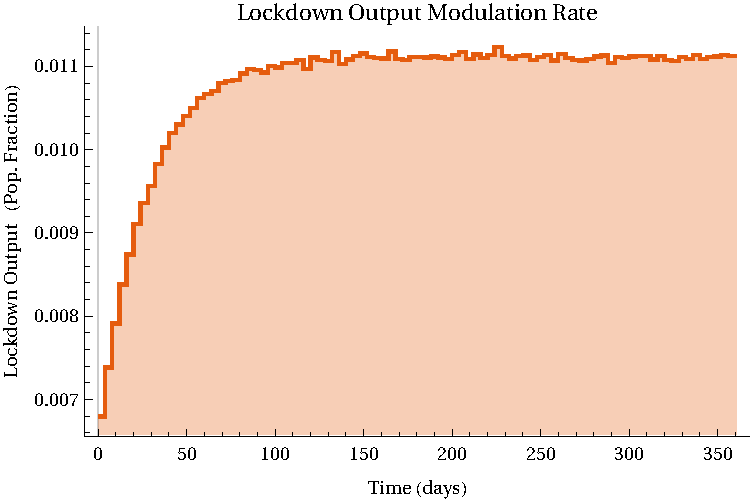
\includegraphics[width=0.7\linewidth]{figs/lockdown_control_signal}
    \caption[Lockdown modulation signal.]{Lockdown modulation signal.
    \href{https://plotly.com/~AdrianSalcedo/56/}
    {https://plotly.com/~AdrianSalcedo/56/}
            to display a electronic viewer.}
    \label{fig:lockdowncontrolsignal}
\end{figure*}

\begin{figure}
    \centering
    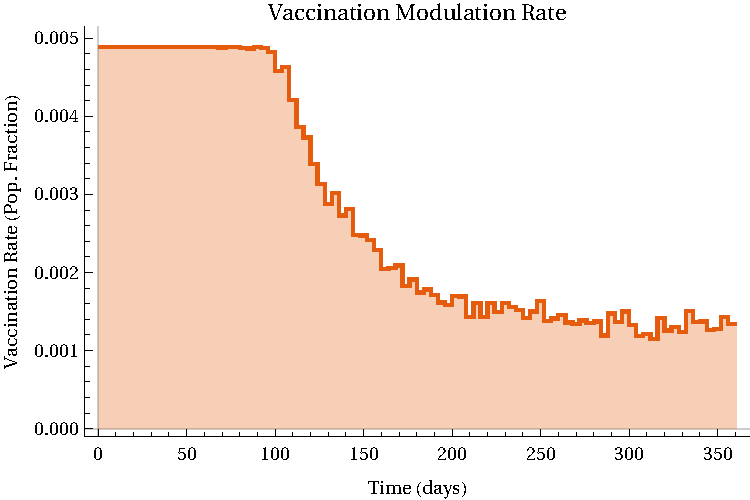
\includegraphics[width=0.7\linewidth]{figs/Vaccination_control_signal}
    \caption[Vaccination rate modulation.]{Vaccination rate modulation.
    \href{https://plotly.com/~AdrianSalcedo/58/}
    {https://plotly.com/~AdrianSalcedo/58/}}
    \label{fig:vaccinationcontrolsignal}
\end{figure}

\begin{figure}[tbh]
    \centering
    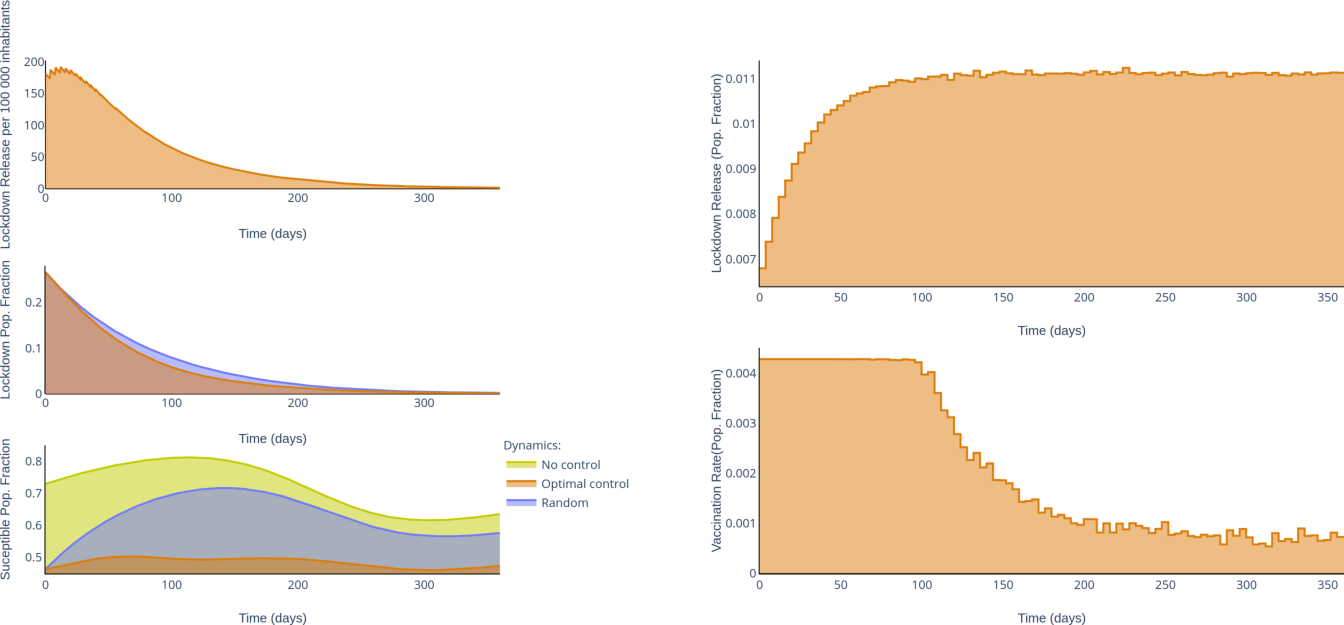
\includegraphics[scale=0.7, keepaspectratio]{%
        ./Figures/Lockdown-Release-Modulation.pdf}
    \caption{Modulation lock down release.
    \href{https://plotly.com/~AdrianSalcedo/60/}
    {https://plotly.com/~AdrianSalcedo/60/}}
    \label{fig:lockdowneffect}
\end{figure}

\begin{figure*}[tbh]
    \centering
    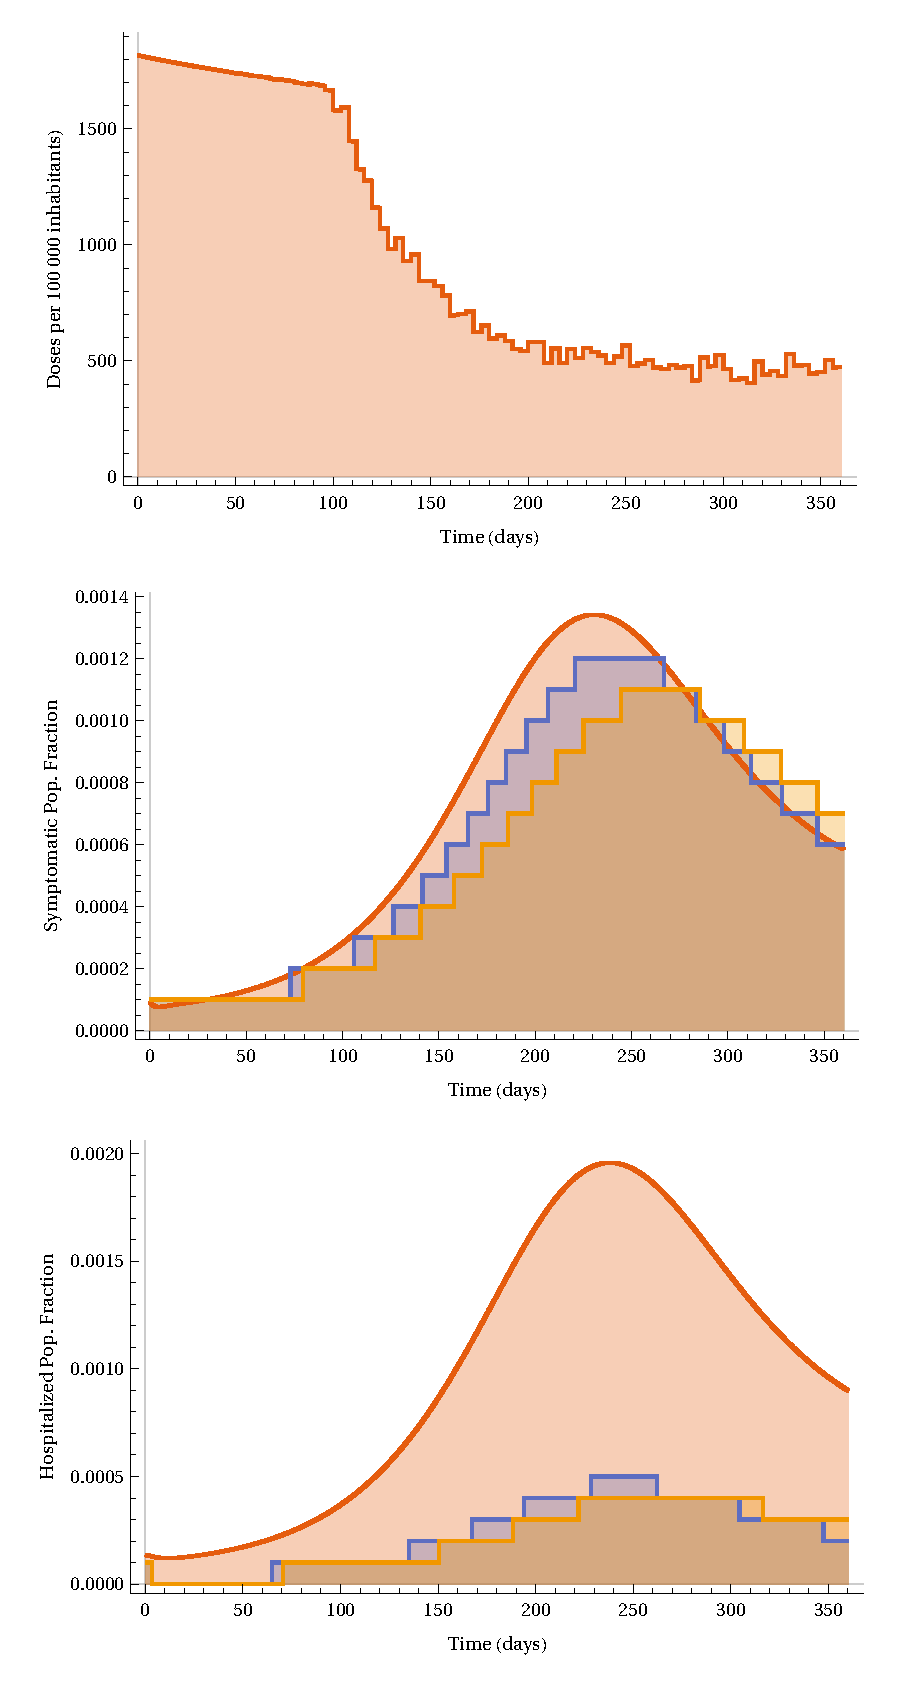
\includegraphics[scale=0.65, keepaspectratio]{figs/VaccinationEffect}
    \caption{Symptomatic Prevalence and Hozpitalization.
        \href{https://plotly.com/~AdrianSalcedo/61/}
        {https://plotly.com/~AdrianSalcedo/61/}}
    \label{fig:vaccinationeffect}
\end{figure*}

    \section{Discussion}
        \label{sec:discussion}
        %!TEX root = main.tex

\paragraph{Statement of principal finding}
    This study illustrated the implications of applying 
combined strategies of lockdown and vaccination to mitigate the curse 
of COVID-19. Our numerical experiments suggest that a combined and 
well-balanced policy between the relaxing times of lockdown and 
vaccine rollout would improve the mitigation of COVID-19 symptomatic 
prevalence and deaths--but with a delicate balance, 
with the economic impact. We obtained lockdown policies that modulate the 
releasing (or holding) of individuals synchronized with and vaccine rollout 
speed as a strategy to mitigate the symptomatic prevalence. 
Our policies captured time windows where it is convenient to modify the 
speed of releasing (or confining) individuals and the rate of vaccine 
administration according to the symptomatic prevalence. 
Here we quantify this convenience by computing a cost functional defined 
by a linear contribution due to the burden of the 
disease\textemdash quantify in DALYs\textemdash and quadratic cost 
of the implementation.

\paragraph{Strengths and weakness of the study}
    %TOPIC SENTENCE
    \begin{CheckList}{Goal}
        \Goal{open}{Argument for Strengths}
            \begin{CheckList}{Task}
                \Task{done}{Piecewise optimal policies}
                \Task{done}{Practical}
                \Task{done}{Modulation between
                    relaxation and inclusion of 
                    population in lockdown}
            \end{CheckList}
    \end{CheckList}

    \paragraph[]{STRENGTHS}
	        We got optimal policies that are practical. 
        Whit practical, we mean those capture actions that can be
	    implemented in the real world. Because the policies rely on 
	    piecewise constant values for a given period (here we use 
	    days), we argue that they are more realistic than policies 
	    based on measurable functions defined on continuos time.
        The policies defined on continuos time could implicate
	    continuous changes of a given action. %
        For example, it results more realistic to administer a 
        fixed number of jabs along with a given date than following 
        a configuration of several doses that would change continuously 
        on the same date.
    
            Besides, we synchronized the trade of between
        lockdown-release, vaccine-rollout but balancing the 
        economic cost.

    \paragraph[]{WEAKNESS}
        \begin{CheckList}{Goal}
            \Goal{open}{Argument for Weakness}
                \begin{CheckList}{Task}
                    \Task{done}{Vaccine Multi-dose.}
                    \Task{done}{Protection only against severe symptoms.}
                    \Task{done}{What expect respect 
                        to the protection against transmission.
                    }
                \end{CheckList}
        \end{CheckList}
  
            One limitation was the assumption of only one vaccine. 
        In almost all countries the vaccination campaigns consider at 
        least two developments. For example, in Mexico the vaccine portfolio 
        (at the day of writing) relies on at least four developments. Moreover, 
        this vaccine portfolio includes developments that differs in the number 
        of required doses. For example, Pfizers require two doses while Cansino 
        Bio only demands one.
        
            Further, we do not face additional vaccine administration 
        requirements as the time between doses or logistics\textemdash 
        each development implies different protocols. Since the approved 
        vaccine's protective efficacy against transmissions of SARS-CoV2 
        remains under study, we do not consider this hypothesis in our
        formulation. We recognize that this parameter would play an 
        important role, which is plausible to consider in future formulations.

    \paragraph{Strengths and weakness in relation to 
        other studies, discussing important differences
        in results
    }
    \todo{citations}
    \paragraph{STRENGTHS}
        \begin{CheckList}{Goal}
            \Goal{open}{Argument for Strengths}
                \begin{CheckList}{Task}
                    \Task{done}{%
                        NPI's optimal Policies with non Vaccination
                        }
                    \Task{done}{%
                        and compare our results.}
                    \Task{done}{What expect respect 
                        to the protection against transmission.
                    }
                    \Task{done}{Optimal Control of Vaccination Rate
                    cite \cite{Libotte2020} among others  and compare our 
                    results
                    }
                \end{CheckList}
        \end{CheckList}
        
        Works like
    \cite{Perkins2020,Palmer2020,Djidjou2020,Asamoah2021,Nabi2021} 
    models NPI's for COVID-19 with optimal control. Some 
    contribution of this list  combines two or more strategies to
    mitigate prevalence and deaths due to SARS-CoV-2. 
    For example, the authors of %
    \cite{Nabi2021} formulates a fractional ODE to model strategies as public
    education, treatment, and management of asymptomatic cases.  
    In \cite{Asamoah2021} Assamoth et al. unfold, an exhaustive analysis
    of the economic cost related with the combined health protocol of 
    physical distancing, media advocacy, mask wearing, hand-washing, 
    lockdown and contact tracing.
    Similarly, \cite{Djomegni2021,Jiang2020,Ullah2020}
    reports optimal policies but with significant emphasis on other aspects 
    related to the spread dynamics of COVID-19. However, the mentioned works 
    developed guidelines based on continuous-time did not optimize or not 
    include vaccination. Our contribution complements these contributions 
    with policies that are piecewise-constant. 
	    
	   Here we argue that our policies give a precise sequence of actions that 
    are feasible for implementation. Further, we calculated the cost and 
    balanced its performance synchronized and balanced with the economic 
    implications.

    \paragraph{WEAKNESS: Static optimization }
        \begin{CheckList}{Goal}
            \Goal{open}{Argument for Weakness}
                \begin{CheckList}{Task}
                    \Task{done}{Allocation.
                        Comment about optimal allocation as a 
                        static optimization problem and cite
                        cite {Bubbar, Buckner, Moore2021}.
                    }
                \end{CheckList}
        \end{CheckList}
    
        On the other hand, this work's limitation was the lack of stratification
    across ages and risk groups. Because DALY's definition depends on this 
    stratification, and the productive sector of an economy is closely related 
    to the workforce, we might prioritize accordingly. However, we see that our 
    result could complement the prioritization policies of relevant works like 
    \cite{Bubar2021,Matrajt2020a,Buckner2020}. In comparison, optimal vaccine 
    prioritization strategies answer the question: Who to vaccine first, we 
    respond when intensifying lockdown (holding) release vaccine rollout. 
    Thus, our contribution would be complementary.

    \paragraph{Meaning of the study: possible explanations 
        and implications for clinicians and policymakers}

        New and more contagious variants of SARS-CoV-2 appeared, 
    and the COVID-19 vaccine supply would be scarce, slow, and 
    complicated for countries like Mexico. Thus we expect three 
    synchronized events: another COVID-19 wave, an
    intensification of the vaccine rollout, and other lockdowns. 
    Here we argued that the above strategies also must be 
    synchronized and consider a delicate balance with the 
    economic impact.

    \paragraph{Unanswered questions and future research}
        
        Despite that NPIs have been implemented in most countries to mitigate 
    COVID-19, these strategies cannot develop immunity. Thus, vaccination 
    becomes the primary pharmaceutical measure. However, this vaccine has to be 
    effective and well implemented in global vaccination programs. Each 
    development implies particular issues--like logistics number of doses, 
    secondary effects, etc. For example, Mexico is administrating vaccines from 
    Pfizer-BioNTech, AstraZeneca, CanSino-Bio, and Sputnik V from Russia. 
    Each of these vaccines implies different requirements for its management, 
    protects with different efficacies, and differs in its number of doses. 
    We believe that this complicated landscape has significant implications in 
    the design of health policies.

        Therefore, we must face new challenges in distribution, stocks, 
    politics, vaccination efforts, and other uncertainties.          
    
    \section*{Data availability}
            \href{https://github.com/%
        SaulDiazInfante/NovelCovid19-OptimalPiecewiseControlModelling.git}{%
        https://github.com/%
        SaulDiazInfante/NovelCovid19-OptimalPiecewiseControlModelling.git}
    \section*{Authors’ contributions}
    \textbf{Gabriel A. Salcedo-Varela}
    Conceptualization,
    Methodology,
    Software,
    Validation,
    Formal analysis,
    Investigation,
    Resources,
    Visualization,
    Project Administration,
    Writing\textendash original draft,
    Writing\textendash review \& editing.

\textbf{F. Pe\'nu\'nuri}
    Methodology,
    Software,
    Validation,
    Formal analysis,
    Investigation,
    Data curation,
    Visualization,
    Supervision,
    Writing\textendash original draft,
    Writing\textendash review \& editing.

\textbf{David Gonz\'alez-S\'anchez:}
    Conceptualization,
    Methodology,
    Formal analysis,
    Writing\textendash original draft,
    Writing\textendash review \& editing.

\textbf{Sa\'ul D\'iaz-Infante:}
    Conceptualization,
    Methodology,
    Formal analysis,
    Writing\textendash original draft,
    Writing\textendash review \& editing.
        Methodology,
    Software,
    Validation,
    Formal analysis,
    Investigation,
    Data curation,
    Visualization,
    Supervision

    \section*{Conflicts of interest}
    The authors have no competing interests.
    
    \appendix
    \section{Existence of optimal policies}
        %!TEX root = main.tex
In this appendix, we show the existence of optimal policies in the class of
{\it piecewise constant policies}. Consider the following cost functional that
we want to minimize
\begin{equation}\label{costFunctional}
  \int_0^T C(X(t),u(t)) dt
\end{equation}
subject to the dynamics
\begin{equation}\label{dynamics}
  \dot{X}(t) = f(X(t),u(t)),  \qquad    0\leq t \leq T,
\end{equation}
and the initial state $X(0)=x_0$. The functions $u:[0,T]\to U$ are called {\it
control polices}, where $U$ is a subset of some Euclidean space.
    %The
    %cost functional \eqref{eqn:cost_functional} and the dynamics
    %\eqref{eqn:vital_dynamics} are particular cases of \eqref{costFunctional}
    %and \eqref{dynamics}, respectively.
%
Let $t_0<t_1<\ldots <t_n$, with
$t_0=0$ and $t_n=T$, be a partition of the interval $[0,T]$.
We consider piecewise constant policies $\tilde{u}$ of the form
\begin{equation}\label{PieceConstCont}
  \tilde{u}(t) = a_j\qquad t_j\leq t < t_{j+1}
\end{equation}
 for $j=0,\ldots,n-1$.
\begin{assumptions}
    We made the following assumptions.
    \begin{enumerate}[label=\textbf{(ASS-\arabic*)}]
        \item
            The function $f$ in the dynamics \eqref{dynamics} is of
            class $C^1$.
        \item
            The cost function $C$ in \eqref{costFunctional} is continuous and
            the set $U$ is compact.
    \end{enumerate}
\end{assumptions}
%

    By Assumption (A-1)\textbf{}, the system
\[
  \dot{X}(t) = f(X(t),a_0), \quad X(0)=x_0, \qquad    0\leq t \leq t_1,
\]
has a unique solution $\tilde{X}_0(t;x_0,a_0)$ which is continuous in
$(x_0,a_0)$; see, for instance \cite{Kong2014}.  Next, put $x_1:=\tilde{X}_0(t_1;x_0,a_0)$ and consider the system
\[
  \dot{X}(t) = f(X(t),a_1), \quad X(t_1)=x_1, \qquad    t_1\leq t \leq t_2,
\]
Again, by Assumption (A-1), the latter system has a unique solution
$\tilde{X}_1(t;x_1,a_1)$ which is
continuous in $(x_1,a_1)$. By following this procedure, we end up having a
recursive solution
\begin{equation*}
  \begin{aligned}
    & \tilde{X}_{n-1}(t;x_{n-1},a_{n-1}),
    \qquad t_{n-1}\leq t \leq T,\\
    & x_{n-1}:=\tilde{X}_{n-2}(t_{n-1};x_{n-2},a_{n-1}),
  \end{aligned}
\end{equation*}
where $\tilde{X}_{n-1}$ is continuous in $(x_{n-1},a_{n-1})$.


For a control $\tilde{u}$ of the form \eqref{PieceConstCont} and the
corresponding solution path $\tilde{X}$, we have
\[
  \int_0^T
    C(\tilde{X}(t),
    \tilde{u}(t)) dt =
      \sum_{j=0}^{n-1}
        \int_{t_j}^{t_{j+1}}
        C(\tilde{X}_j(t),a_j) dt.
\]
Notice that each $\tilde{X}_j$ is a continuous function of $(a_0,\ldots,a_j)$
and $x_0$.

By Assumption (A-2), the mapping
\[
  (a_0,\ldots,a_{n-1})
  \mapsto
  \sum_{j=0}^{n-1}
  \int_{t_j}^{t_{j+1}} C(\tilde{X}_j(t),a_j) dt
\]
is continuous. Since each piecewise constant policy $\tilde{u}$ of the form
\eqref{PieceConstCont} can be identified with the vector $(a_0,\ldots,a_{n-1})$
in the compact set $U\times\cdots\times U$, the functional
\eqref{costFunctional} attains its minimum in the class of piecewise constant
policies.

    The cost functional \eqref{eqn:cost_functional} and the dynamics
\eqref{eqn:base_dynamics} are particular cases of \eqref{costFunctional} and
\eqref{dynamics}, respectively, and satisfy Assumptions (A-1) and (A-2). Then
there exists an optimal vaccination policy of the form \eqref{PieceConstCont}.
        \bibliography{NovelCovid19.bib}
        %\bibliographystyle{plain}
    \bibliographystyle{elsarticle-num}
\end{document}
